%% ======================================================================
%%  FMC manual -- MASTER DOCUMENT
%%  Edit this file.  Both the PDF and the README.md are generated from it:
%%     bash docs/build_manual.sh          (PDF + README.md)
%%  Keep to the LaTeX subset described in docs/README_build.md so that
%%  pandoc can convert it to GitHub Markdown.
%% ======================================================================
\documentclass[11pt,a4paper,english]{article}
\usepackage{lmodern}
\usepackage{mathpazo}
\usepackage{avant}
\usepackage[T1]{fontenc}
\usepackage{textcomp}
\usepackage[utf8]{inputenc}
\usepackage{underscore}% allows line breaks after underscores (long parameter names in narrow table cells)
\DeclareUnicodeCharacter{2212}{\ensuremath{-}}
\pagestyle{plain}
\setcounter{secnumdepth}{2}
\setcounter{tocdepth}{2}
\usepackage{xcolor}
\usepackage{babel}
\usepackage{float}
\usepackage{calc}
\usepackage{amsmath}
\usepackage{graphicx}
\usepackage{longtable,booktabs,array}
\usepackage{etoolbox}
\AtBeginEnvironment{longtable}{\small}
\usepackage{listings}
\lstset{basicstyle=\ttfamily\small, frame=shadowbox, rulesepcolor=\color{black!60},
  breaklines=true, breakatwhitespace=false, showstringspaces=false, keepspaces=true,
  xleftmargin=0.6em, xrightmargin=0.6em, aboveskip=0.8em, belowskip=0.6em}
\usepackage[authoryear]{natbib}
\usepackage[bookmarks=true,bookmarksnumbered=false,bookmarksopen=false,
 breaklinks=false,pdfborder={0 0 0},pdfborderstyle={},backref=false,colorlinks=true]
 {hyperref}
\hypersetup{pdftitle={Focal mechanisms managing, classification and plot program. The FMC Manual},
 pdfauthor={Jos\'e A. \'Alvarez-G\'omez}}

\makeatletter
\newcommand{\noun}[1]{\textsc{#1}}
\numberwithin{equation}{section}
\@ifundefined{date}{}{\date{}}
\setlength{\parskip}{\medskipamount}
\setlength{\parindent}{0pt}
\setlength{\emergencystretch}{3em}
\makeatother

\newcommand{\fmcversion}{1.10}
\newcommand{\fmcdate}{September 2026}

\begin{document}
\title{\texttt{FMC}\\
A program to manage, classify, cluster and plot focal mechanism data\\
{\small\texttt{\noun{version \fmcversion, \fmcdate}}}}
\author{\noindent José A. Álvarez-Gómez\\
{\small\emph{Faculty of Geology. Universidad Complutense de Madrid}}}

\maketitle
\vspace{10cm}

\begin{flushleft}% front-page license note (left out of the README)
\rule[0.5ex]{1\columnwidth}{0.8pt}

\IfFileExists{figures/CreativeCommons_88x31.png}{
\includegraphics[scale=0.6]{figures/CreativeCommons_88x31.png}\par}{}

{\small This text is distributed under the Creative Commons License:}\\
{\small Attribution-NonCommercial-ShareAlike 4.0 International (\href{https://creativecommons.org/licenses/by-nc-sa/4.0/legalcode}{CC BY-NC-SA 4.0}) }{\small\par}
\end{flushleft}

\newpage{}

\tableofcontents{}

\newpage{}

\section*{Acknowledgments}

I have been using different versions of this program during the last
decade. Initially I reworked some of the \citet{gasp03} FORTRAN subroutines
on Matlab in order to obtain all the focal mechanism parameters from
the Harvard CMT \texttt{psmeca} formatted catalog. During my research
on seismotectonics I started to use the \citet{froh92} diagram, but
after \citet{kaga05} I decided to try the \citet{kave96} one. From
the original Matlab program I jumped to the Free Software world adapting
it to Octave. The program only produced the x and y positions of the
events and all the plotting was done by means of GMT \citep{gmt}.

Some colleagues wanted to use the diagram for their work, but they
were not familiar with GMT, so I decided to make a big improvement
in the program to make it easy to use, distributable and with plotting
support. I choose to program it in Python with the following basic
ideas:
\begin{enumerate}
\item It should be called from the terminal or the command line in order
to be incorporated into shell scripts
\item It should behave like any other shell unix tool, compatible with redirection,
piping and ASCII format
\item it should be compatible with the GMT \texttt{psmeca} formats to allow
the mapping of the focal mechanisms
\item It should has the option to produce a \citet{kave96} type classification
diagram
\end{enumerate}
Part of the programming was done during my happy days as Ph.D. candidate
at the UCM; so I have to acknowledge the UCM scholarship that allowed
me to start my scientific career.

I would like to thank the beta testers Jorge L. Giner-Robles and Alberto
Jiménez-Díaz for their comments and suggestions. Dr. Andrei Bala (National
Institute for Earth Physics, Romania) has tested different versions
and suggested several improvements.

\bigskip{}

If you use \texttt{FMC}, and consider it appropriate, you can acknowledge
it by citing the following reference:
\begin{itemize}
\item Álvarez-Gómez, J. A. (2019). FMC---Earthquake focal mechanisms data
management, cluster and classification. SoftwareX, 9, 299-307. \url{https://doi.org/10.1016/j.softx.2019.03.008}
\end{itemize}
You should cite the SoftwareX paper if you are using the last version
of the program with clustering and several plot customization options.

BibTeX entry of the SoftwareX paper:

\begin{lstlisting}
@article{AlvarezGomez2019FMC,
  author  = {{\'A}lvarez-G{\'o}mez, Jos{\'e} A.},
  title   = {{FMC}---Earthquake focal mechanisms data management, cluster and classification},
  journal = {SoftwareX},
  volume  = {9},
  pages   = {299--307},
  year    = {2019},
  doi     = {10.1016/j.softx.2019.03.008}
}
\end{lstlisting}

\newpage{}

\part{The manual}

\section{Introduction}

This is the user manual for the program \texttt{FMC} (from Focal Mechanisms
Classification). This program was originally developed on Python 2.7.3
and adapts some of the \citet{gasp03} FORTRAN routines to obtain
the different parameters of the earthquake focal mechanisms depending
on the input format. Since version 1.3 it is compatible with Python
3. Several output formats are eligible, clustering analysis of the
data can be performed and a classification diagram for the focal mechanisms
is produced; a source-type diagram of the moment tensors can also be plotted. The default input and output formats are the same used
by the GMT program \texttt{psmeca} in order to make the program integration
easiest and facilitate the mapping of the data.

The program basically takes the focal mechanisms data, computes the
different parameters that can be obtained, classifies each focal mechanism
in one of seven possible types, perform a clustering analysis of the
data if it is required by the user and optionally outputs the parameters
in different formats and generates a classification diagram from the
input data.

\section{Versions}
\label{sec:versions}

\paragraph{1.10}

New features:
\begin{itemize}
\item New parameter \texttt{Gamma}: CLVD index of \citet{kaga85}, computed from the deviatoric eigenvalues. It is included in the \texttt{ALL} output after \texttt{fclvd}, so the following columns move one position.
\item The left label of the source-type diagram is now ``CLVD (+)'', and the symbol of maximum magnitude of its legend keeps its position.
\end{itemize}
Changes:
\begin{itemize}
\item The CLVD ratio \texttt{fclvd} is computed from the deviatoric eigenvalues and follows the definition of \citet{froh99}: it is positive for tension-dominated CLVD, as in the source-type diagram and in \citet{vavr15}. Its sign is opposite to that of versions 1.8.1 to 1.9.1 (section~\ref{sec:parameters-computed-by-fmc}).
\end{itemize}

\paragraph{1.9.1}

Bug fixes:
\begin{itemize}
\item Labels (\texttt{-pa}) with NumPy 2.x; source-type diagram (\texttt{-pd}) with a single event, equal magnitudes or \texttt{PT} input; no \texttt{NaN} for mechanisms at the centre of the classification diagram.
\item \texttt{-pg} without a value uses its default (10); \texttt{-pc} with a non-numeric parameter (such as an alphanumeric \texttt{ID}) gives a warning and white symbols; the default plot title is the file name without path or extension.
\item Clear error message when the clustering methods \texttt{centroid}, \texttt{median} or \texttt{ward} are used with a non-Euclidean metric.
\item Magnitude legend formatted as 8.0 (previously 8.); the text label of the source-type diagram is no longer clipped; the version number shown by \texttt{-h} is correct.
\end{itemize}

\paragraph{1.9}

New features:
\begin{itemize}
\item The symbol sizes of the diagrams are scaled to the magnitude range of the input data; the legend shows the minimum and maximum Mw.
\end{itemize}

\paragraph{1.8.1}

Changes:
\begin{itemize}
\item The CLVD ratio \texttt{fclvd} follows the definition of \citet{giar84}: it is now a signed value between $-0.5$ and $+0.5$ (previously its absolute value, as in \citealp{froh92}). The sign convention was reversed in version 1.10.
\end{itemize}

\paragraph{1.8}

New features:
\begin{itemize}
\item New output parameter \texttt{fiso}: ratio between the isotropic component and the scalar seismic moment.
\end{itemize}

\paragraph{1.7}

New features:
\begin{itemize}
\item New input format \texttt{PT}: orientation of the P and T axes, for instance strain axes obtained from fault-slip analysis.
\item New parameter \texttt{data1}: a free numeric value carried with the \texttt{PT} input, usable to colour or label the symbols.
\end{itemize}

\paragraph{1.6}

New features:
\begin{itemize}
\item Source-type diagram of \citet{huds89} (flag \texttt{-pd}) and new parameters \texttt{u\_Hudson} and \texttt{v\_Hudson}.
\end{itemize}

\paragraph{1.5.1}

Bug fixes:
\begin{itemize}
\item Correction in the data reading routine (\texttt{genfromtxt}).
\end{itemize}
Changes:
\begin{itemize}
\item Adjustment of the T and B axes labels in the diagram.
\end{itemize}

\paragraph{1.5}

Bug fixes:
\begin{itemize}
\item Several corrections.
\end{itemize}
New features:
\begin{itemize}
\item Warning when a non-numeric parameter is used to fill the symbols.
\end{itemize}

\paragraph{1.4}

New features:
\begin{itemize}
\item Custom plot title (flag \texttt{-pt}).
\end{itemize}
Bug fixes:
\begin{itemize}
\item Several corrections.
\end{itemize}

\paragraph{1.3}

New features:
\begin{itemize}
\item Added support for Python 3.
\item Added new base diagram labels and tick marks.
\item Added symbol labeling.
\item Added gridlines plotting.
\item Added isotropic component output.
\end{itemize}

\paragraph{1.2}

New features:
\begin{itemize}
\item Added slip sense and plunge parameters for each focal mechanism nodal
plane.
\end{itemize}

\paragraph{1.1}

New features:
\begin{itemize}
\item New custom output parsing. The user can choose between the standard
predefined output or any parameters in any order.
\item Added a header with the parameter name in the output.
\item Added symbol coloring.
\item Added hierarchical clustering with several methods and options.
\end{itemize}

\paragraph{1.01}

New features:
\begin{itemize}
\item Column number is now included in the header of the output file with
all the parameters.
\end{itemize}
Bug fixes:
\begin{itemize}
\item Error in the nd2ar function to obtain the tensor components from the
nodal planes.
\end{itemize}

\paragraph{1.0}

Initial release of \texttt{FMC} with basic plotting function and focal
mechanisms management.

\section{Installation}

\texttt{FMC} has been programmed in Python 3 and uses several
common python libraries: \texttt{sys}, \texttt{argparse}, \texttt{os},
\texttt{NumPy}, \texttt{SciPy} and \texttt{matplotlib}. Depending on your operative
system and Python installation you could need to install some of the
libraries manually.

For \textbf{Windows} and \textbf{Mac} users a good starting point
is the installation of predefined packages. From \href{http://www.SciPy.org}{www.SciPy.org}
you can download program packages that includes\texttt{ Python}, \texttt{NumPy},
\texttt{SciPy} and \texttt{matplotlib}, as well as other modules and IDEs. With one
of these packages installed \texttt{FMC} should work properly.

For \textbf{Linux} users all the required software can be easily installed
through your favorite distribution repository (the python modules\texttt{
sys}, \texttt{argparse} and \texttt{os} are usually installed with
the default python installation).

The libraries can also be installed with \texttt{pip}: \texttt{pip install numpy scipy matplotlib}.

\texttt{FMC} is formed by three files that must be kept in the same directory: \texttt{FMC.py} (main program), \texttt{functionsFMC.py} (computational functions) and \texttt{plotFMC.py} (plotting functions). The repository includes a small test file, \texttt{jap\_select.dat}, with 16 large earthquakes from Japan in Global CMT format. The command \texttt{FMC.py jap\_select.dat} should print the 16 events with a new column with their rupture type.

\section{Usage}

The user interface is as simple as a ``command line'', or a ``terminal''.
I decided to keep the program interface as simple as possible so it can be integrated
into scripts with other programs such as \href{http://www.soest.hawaii.edu/gmt5/}{GMT},
\texttt{AWK (or \href{http://www.gnu.org/software/gawk/}{gawk})}
or any other tool running from a shell or script (in *nix) or a
command window or batch file (in Windows/DOS). In the following the
commands are written assuming that your python installation recognizes
automatically the python format. In some systems, depending on your
personal configuration, you will need to call first Python (like ``\texttt{python
FMC.py...}'' or ''\texttt{python3 FMC.py...}'') or in a *nix
system with the ``./'' needed to execute a script (like \texttt{./FMC.py
...}).

In *nix you will need to give execution permission to the program:

\begin{lstlisting}[language=bash]
chmod +x FMC.py
\end{lstlisting}

To run \texttt{FMC} on a file simply type in the terminal:

\begin{lstlisting}[language=bash]
FMC.py input-file.dat
\end{lstlisting}

By default \texttt{FMC} will read the input file as a \texttt{psmeca}
Centroid Moment Tensor (CMT) format (in Harvard convention). This
kind of file can be downloaded directly from \href{http://www.globalcmt.org/}{Global CMT}.
The output will be shown on the screen in\texttt{ psmeca} CMT format
so it can be directly pipe into \texttt{psmeca:}

\begin{lstlisting}[language=bash]
FMC.py input-file.dat | psmeca -R {...etc}
\end{lstlisting}

Or stored as an ASCII file:

\begin{lstlisting}[language=bash]
FMC.py input-file.dat > output-file.dat
\end{lstlisting}

In this case \texttt{FMC} will add a new column at the end of each
register with the focal mechanism type.

Alternatively the input file can be a single plane in \citet{aki80}
convention (Right Hand Rule for the plane orientation, and rakes from
0 to 180 in reverse faults and 0 to -180 in normal faults, 0 for left-lateral
and $\pm$180 for right-lateral). This format is also compatible with
\texttt{psmeca}.

\subsection{Input}
\label{sec:input}

\texttt{FMC} input can be given as an ASCII file or as standard input, from a pipe (``|'') or a redirection (``<''). The following codes are then equivalent:

\begin{lstlisting}[language=bash]
FMC.py input-file.dat

cat input-file.dat | FMC.py

FMC.py < input-file.dat
\end{lstlisting}

If no input is given, then \texttt{FMC} will show the on-screen help.

The\textbf{ }input format is specified with the optional flag ``\texttt{-i}'', and the possible values are:
\begin{description}
\item[CMT] Harvard Centroid Moment Tensor (by default):\\
\texttt{[longitude, latitude, depth, mrr, mtt, mff, mrt, mrf, mtf, Exponent (dyn-cm), X plot, Y plot (for GMT), ID]}
\item[AR] Aki and Richards one plane convention:\\
\texttt{[longitude, latitude, depth, strike, dip, rake, magnitude (Mw), X plot, Y plot (for GMT), ID]}
\item[P] Both nodal planes and scalar seismic moment:\\
\texttt{[longitude, latitude, depth, strike A, dip A, rake A, strike B, dip B, rake B, Scalar seismic moment mantissa, Exponent (dyn-cm), X plot, Y plot (for GMT), ID]}
\item[PT] Orientation of the P and T axes:\\
\texttt{[longitude, latitude, trend P, plunge P, trend T, plunge T, data1, X plot, Y plot (for GMT), ID]}
\end{description}
The data are whitespace-separated columns, one event per line. Lines starting with \texttt{\#} are ignored, so the header written by \texttt{FMC} does not disturb a later reading. Every line must have the exact number of columns of the chosen format, and the \texttt{ID} must not contain spaces. With the \texttt{P} format the axes and the moment tensor are computed from plane A.

The \texttt{PT} format is intended for tensors that are not earthquake focal mechanisms, such as the shortening (P) and extension (T) axes obtained from fault-slip inversion; the P and T axes must be orthogonal. \texttt{data1} is any numeric value (a site number, the number of faults, a misfit...) that can be used to colour (\texttt{-pc data1}) or label (\texttt{-pa data1}) the symbols or to perform the clustering (\texttt{-ci data1}). As there is no depth or magnitude information \texttt{FMC} assigns depth 0, $M_0=10^{20}$ dyn$\cdot$cm and Mw 8.0.

\subsection{Output}
\label{sec:output}

\texttt{FMC} output format can be selected among the following options with the flag ``\texttt{-o}'':
\begin{description}
\item[CMT] Harvard Centroid Moment Tensor (\texttt{psmeca} compatible):\\
\texttt{[longitude, latitude, depth, mrr, mtt, mff, mrt, mrf, mtf, Exponent (dyn·cm), X plot, Y plot (for GMT), ID, TYPE]}
\item[P] Focal mechanism both nodal planes (\texttt{psmeca} compatible):\\
\texttt{[longitude, latitude, depth, strike A, dip A, rake A, strike B, dip B, rake B, Scalar seismic moment mantissa, Exponent (dyn·cm), X plot, Y plot (for GMT), ID, TYPE]}
\item[AR] Focal mechanism one plane (\texttt{psmeca} compatible):\\
\texttt{[longitude, latitude, depth, strike, dip, rake, magnitude (Mw), X plot, Y plot (for GMT), ID, TYPE]}
\item[K] Kaverina diagram position for plotting outside FMC:\\
\texttt{[X Kaverina diagram, Y Kaverina diagram, Mw, Depth, ID, TYPE]}
\item[ALL] All the parameters obtained:\\
\texttt{[longitude, latitude, depth, mrr, mtt, mff, mrt, mrf, mtf, Exponent (dyn·cm), Scalar seismic moment (dyn·cm), Mw, strike A, dip A, rake A, strike B, dip B, rake B, Slip trend A, Slip plunge A, Slip trend B, Slip plunge B, P trend, P plunge, B trend, B plunge, T trend, T plunge, fclvd, Gamma, Isotropic component, Isotropic ratio, u Hudson, v Hudson, X Kaverina diagram, Y Kaverina diagram, ID, TYPE]}
\item[CUSTOM] In case you need any focal mechanism parameters in any order you can use the CUSTOM option and give the requested parameters in any order using the flag ``\texttt{-of}''. The output parameters need to be listed separated by commas. The accepted parameters names are listed below, and can be seen on the terminal using \texttt{FMC.py -helpFields}

\begin{description}
\item[lon] longitude
\item[lat] latitude
\item[dep] depth
\item[mrr] mrr centroid moment tensor component
\item[mtt] mtt centroid moment tensor component
\item[mff] mff centroid moment tensor component
\item[mrt] mrt centroid moment tensor component
\item[mrf] mrf centroid moment tensor component
\item[mtf] mtf centroid moment tensor component
\item[mant] mantissa of the seismic moment tensor
\item[expo] exponent of the seismic moment tensor
\item[Mo] Scalar seismic moment
\item[Mw] Moment (or Kanamori) magnitude
\item[strA] Strike of nodal plane A
\item[dipA] Dip of nodal plane A
\item[rakeA] Rake of nodal plane A
\item[strB] Strike of nodal plane B
\item[dipB] Dip of nodal plane B
\item[rakeB] Rake of nodal plane B
\item[slipA] Trend of the slip vector of plane A
\item[plungA] Plunge of slip vector of plane A
\item[slipB] Trend of the slip vector of plane B
\item[plungB] Plunge of slip vector of plane B
\item[trendp] Trend of P axis
\item[plungp] Plunge of P axis
\item[trendb] Trend of B axis
\item[plungb] Plunge of B axis
\item[trendt] Trend of T axis
\item[plungt] Plunge of T axis
\item[fclvd] Compensated linear vector dipole ratio (positive for tension; section~\ref{sec:parameters-computed-by-fmc})
\item[Gamma] CLVD index of \citet{kaga85}
\item[iso] Isotropic component of the Moment Tensor
\item[fiso] Ratio between the isotropic component and the scalar seismic moment
\item[u\_Hudson] u position on the source-type diagram
\item[v\_Hudson] v position on the source-type diagram
\item[x\_kav] x position on the Kaverina diagram
\item[y\_kav] y position on the Kaverina diagram
\item[ID] ID of the event
\item[clas] Focal mechanism rupture type
\item[posX] X plotting position for GMT psmeca
\item[posY] Y plotting position for GMT psmeca
\item[clustID] Cluster number (0 if no clustering analysis is done)
\item[data1] Free numeric value of the \texttt{PT} input (0 otherwise)
\end{description}
\end{description}
All the output formats start with a header line, beginning with \texttt{\#}, with the name of each column. Except \texttt{CUSTOM}, all of them add the rupture type (\texttt{TYPE}) as last column, and the cluster number (\texttt{Cluster\_ID}) when a clustering analysis is done. In the \texttt{CMT} output the tensor components are rescaled to the exponent of the computed scalar moment, so the output exponent may differ from the input one.

Columns of the \texttt{ALL} output (useful to select fields with \texttt{awk}):
{\tiny
\begin{longtable}
{p{0.01\linewidth}p{0.27\linewidth}p{0.01\linewidth}p{0.2\linewidth}p{0.01\linewidth}p{0.32\linewidth}}
\toprule
\textbf{\#} & \textbf{Header} & \textbf{\#} & \textbf{Header} & \textbf{\#} & \textbf{Header} \\
\midrule
\endhead
1 & Longitude & 14 & Dip\_A & 27 & Trend\_T \\
2 & Latitude & 15 & Rake\_A & 28 & Plunge\_T \\
3 & Depth\_(km) & 16 & Strike\_B & 29 & fclvd \\
4 & mrr & 17 & Dip\_B & 30 & Gamma \\
5 & mtt & 18 & Rake\_B & 31 & Isotropic \\
6 & mff & 19 & Slip\_trend\_A & 32 & Iso\_ratio \\
7 & mrt & 20 & Slip\_plunge\_A & 33 & u\_Hudson \\
8 & mrf & 21 & Slip\_trend\_B & 34 & v\_Hudson \\
9 & mtf & 22 & Slip\_plunge\_B & 35 & X\_Kaverina \\
10 & Exponent\_(dyn-cm) & 23 & Trend\_P & 36 & Y\_Kaverina \\
11 & Seismic\_moment\_Mo & 24 & Plunge\_P & 37 & ID \\
12 & Magnitude\_Mw & 25 & Trend\_B & 38 & rupture\_type \\
13 & Strike\_A & 26 & Plunge\_B & 39 & Cluster\_ID (if clustering) \\
\bottomrule
\end{longtable}
}

\subsubsection{Examples of use}

\textbf{Obtaining nodal planes from moment tensor}

Command:

\begin{lstlisting}[language=bash]
echo -2.54 37.09 12 -3.4669 -2.0652 5.5321 6.2368 -1.8004 -5.1775 22 X Y ID | FMC.py -o P
\end{lstlisting}

Result:

\begin{lstlisting}
#Longitude Latitude Depth_(km) Strike_A Dip_A Rake_A Strike_B Dip_B Rake_B Seismic_moment_mantissa Exponent_(dyn-cm) X_position(GMT) Y_position(GMT) ID rupture_type
-2.54 37.09 12.0 190.925 42.4899 -20.9735 296.709 76.0089 -130.541 9.611967 22.0 X Y ID N-SS
\end{lstlisting}

\textbf{Obtaining moment tensor from one nodal plane}

Command:

\begin{lstlisting}[language=bash]
echo -2.54 37.09 12 190.925 42.4899 -20.9735 4.6 X Y ID | FMC.py -i AR -o CMT
\end{lstlisting}

Result:

\begin{lstlisting}
#Longitude Latitude Depth_(km) mrr mtt mff mrt mrf mtf Exponent_(dyn-cm) X_position(GMT) Y_position(GMT) ID rupture_type
-2.54 37.09 12.0 -3.56563 -2.21928 5.78491 6.70126 -1.61249 -5.19047 22.0 X Y ID N-SS
\end{lstlisting}

\textbf{Obtaining all the parameters from the moment tensor}

Command:

\begin{lstlisting}[language=bash]
echo -2.54 37.09 12 -3.4669 -2.0652 5.5321 6.2368 -1.8004 -5.1775 22 X Y ID | FMC.py -o ALL
\end{lstlisting}

Result:

\begin{lstlisting}
#Longitude Latitude Depth_(km) mrr mtt mff mrt mrf mtf Exponent_(dyn-cm) Seismic_moment_Mo Magnitude_Mw Strike_A Dip_A Rake_A Strike_B Dip_B Rake_B Slip_trend_A Slip_plunge_A Slip_trend_B Slip_plunge_B Trend_P Plunge_P Trend_B Plunge_B Trend_T Plunge_T fclvd Gamma Isotropic Iso_ratio u_Hudson v_Hudson X_Kaverina Y_Kaverina ID rupture_type
-2.54 37.09 12.0 -3.4669 -2.0652 5.5321 6.2368 -1.8004 -5.1775 22.0 9.61197e+22 4.6 190.925 42.4899 -20.9735 296.709 76.0089 -130.541 206.709 -13.9911 100.925 -47.5101 167.141 43.8185 308.393 39.1024 56.0979 20.5155 0.0445259 0.117979 -1398100.0 -1.45454e-17 -0.0890517 0.0 -0.243839 0.0899979 ID N-SS
\end{lstlisting}

\textbf{Obtaining all the parameters from CMT input file and storing to an ASCII file}

Command:

\begin{lstlisting}[language=bash]
FMC.py -o ALL jap_select.dat > Japan_parameters.dat
\end{lstlisting}

\textbf{Using CUSTOM output to obtain event location and slip vector of both nodal planes}

Command:

\begin{lstlisting}[language=bash]
echo -2.54 37.09 12 -3.4669 -2.0652 5.5321 6.2368 -1.8004 -5.1775 22 X Y ID | FMC.py -o CUSTOM -of lon,lat,slipA,plungA,slipB,plungB
\end{lstlisting}

Result:

\begin{lstlisting}
#Longitude Latitude Slip_trend_A Slip_plunge_A Slip_trend_B Slip_plunge_B
-2.54 37.09 206.709 -13.9911 100.925 -47.5101
\end{lstlisting}

\textbf{Obtaining the CLVD parameters of a catalogue}

Command:

\begin{lstlisting}[language=bash]
FMC.py -o CUSTOM -of ID,Mw,fclvd,Gamma,clas jap_select.dat
\end{lstlisting}

Result (first events):

\begin{lstlisting}
#ID Magnitude_Mw fclvd Gamma rupture_type
032378C 7.6 0.00882022 0.0230146 R
052683A 7.7 0.122769 0.33196 R
110189E 7.4 0.050104 0.133035 R
071293B 7.7 0.0604748 0.161154 R
\end{lstlisting}

\textbf{Obtaining nodal planes and B axis from P and T axes (PT input)}

Command:

\begin{lstlisting}[language=bash]
FMC.py -i PT -o CUSTOM -of ID,trendb,plungb,strA,dipA,rakeA,strB,dipB,rakeB,clas,data1 pt_example.dat
\end{lstlisting}

Result:

\begin{lstlisting}
#ID Trend_B Plunge_B Strike_A Dip_A Rake_A Strike_B Dip_B Rake_B rupture_type data1
S1 350.0 80.0 214.561 82.947 -7.10708 305.439 82.947 -172.893 SS 12.0
S2 200.0 85.0 155.109 86.4667 -176.46 64.8908 86.4667 -3.54002 SS 25.0
S3 315.0 1.59028e-15 315.0 25.0 -90.0 135.0 65.0 -90.0 N 8.0
S4 210.0 7.95139e-15 210.0 15.0 90.0 30.0 75.0 90.0 R 40.0
S5 120.0 50.0 337.454 62.966 -30.6821 82.5463 62.966 -149.318 SS-N 30.0
\end{lstlisting}

\textbf{Using an FMC output as input}

The extra column with the rupture type must be removed first, for instance with \texttt{awk}:

\begin{lstlisting}[language=bash]
FMC.py -o AR jap_select.dat | awk '{$NF=""; print}' | FMC.py -i AR -o CMT
\end{lstlisting}

\subsection{Plot}
\label{sec:plot}

Optionally \texttt{FMC} will produce a classification diagram. \texttt{FMC}
uses \texttt{matplotlib} libraries and can generate figures in different
formats (emf, eps, jpeg, jpg, pdf, png, ps, raw, rgba, svg, svgz,
tif, tiff). The format is determined automatically from the plot file
name extension.

The diagram uses the \citet{kave96} projection technique, used also
by \citet{kaga05}; but incorporating a classification similar to
the geological conceptual classification of faults. The earthquakes
are classified into seven types according to the values of the P,
T and B Centroid Moment Tensor axes following a simple algorithm (Figure
\ref{fig_flow}), and are represented conveniently on the Kaverina
diagram (Figure \ref{fig_diagram}). This classification is very similar
to the used by \citet{EPRI}.

\begin{figure}[H]
\centering
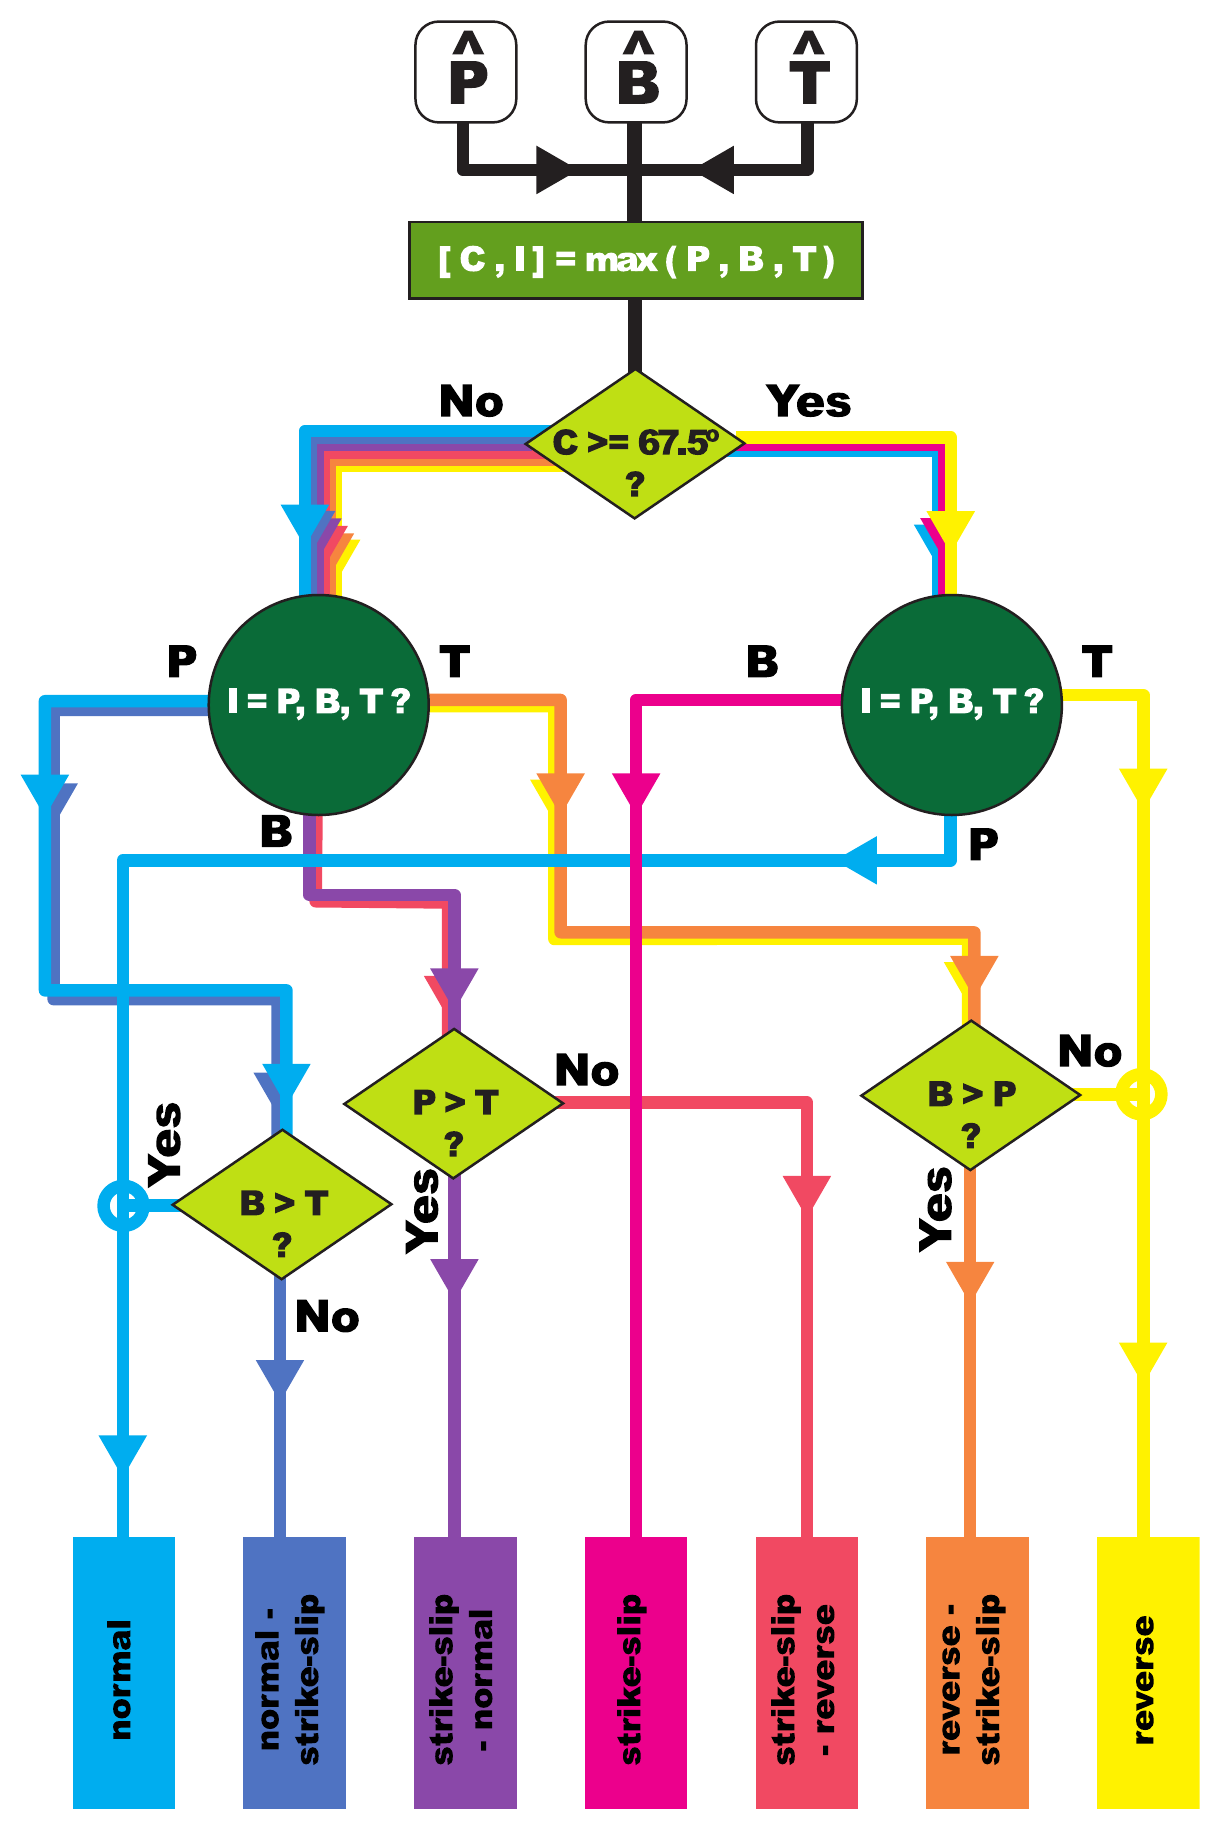
\includegraphics[width=0.62\textwidth]{figures/fig_classification_flowchart.png}
\caption{Focal mechanism classification algorithm flow chart.}
\label{fig_flow}
\end{figure}

\begin{figure}[H]
\centering
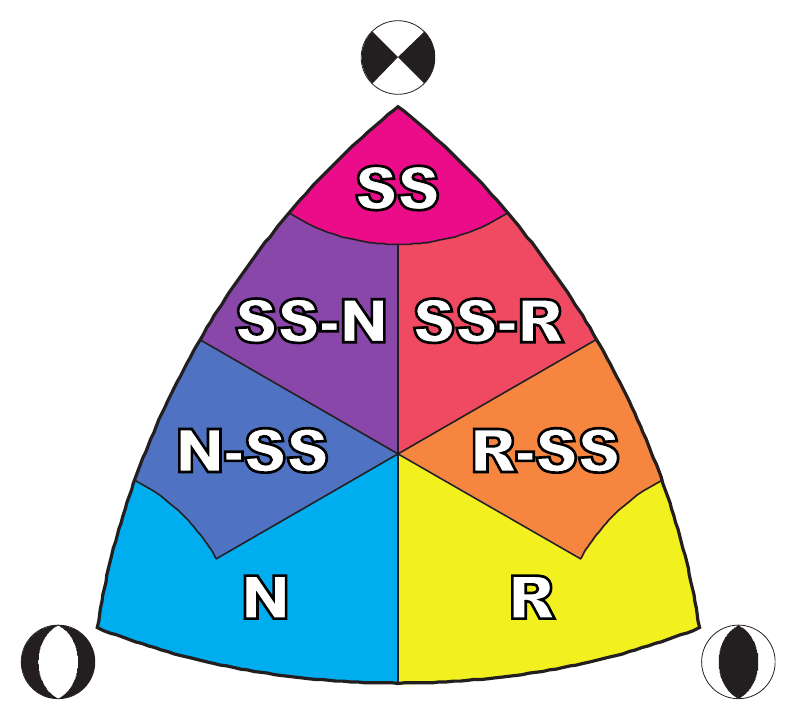
\includegraphics[width=0.50\textwidth]{figures/fig_classification_diagram.png}
\caption{Classification diagram. N: Normal; N-SS: Normal - Strike-slip; SS-N:
Strike-slip - Normal; SS: Strike-slip; SS-R: Strike-slip - Reverse;
R-SS: Reverse - Strike-slip; R: Reverse.}
\label{fig_diagram}
\end{figure}

The size of the symbols is proportional to the magnitude, scaled between the minimum and maximum Mw of the data, which are shown in the legend. \texttt{FMC} uses several flags in order to customize the plot.
\begin{description}
\item[\texttt{-p}] This flag activates the plotting. It must be followed by the name of the figure file that will be produced. The name used for the file (without the extension) is used as title for the plot, unless a different one is given with \texttt{-pt}.
\item[\texttt{-pd}] This flag plots the source-type diagram of \citet{huds89} (section~\ref{sec:the-source-type-diagram}) in the given file. The flags \texttt{-pc}, \texttt{-pa} and \texttt{-pt} also work with this diagram.
\item[\texttt{-pc}] With this flag the user specifies the parameter that is used to fill the symbols. A color palette is produced with the range of the selected parameter values. The parameter must be numeric; otherwise \texttt{FMC} gives a warning and draws white symbols.
\item[\texttt{-pg}] This flag is used to plot gridlines with the specified grid spacing (10 degrees if no value is given).
\item[\texttt{-pa}] This flag is used to annotate the symbols with a certain parameter.
\item[\texttt{-pt}] Plot title. \texttt{-pt\ "\ "} removes the title.
\end{description}
With \texttt{-pc} and \texttt{-pa} the parameters must be given with its corresponding internal name as listed in section \ref{sec:output}.

\subsubsection{Examples of use}

\textbf{Plotting data from standard input}

Command:

\begin{lstlisting}[language=bash]
echo -2.54 37.09 12 -3.4669 -2.0652 5.5321 6.2368 -1.8004 -5.1775 22 X Y ID | FMC.py -p "My data.png"
\end{lstlisting}

\begin{figure}[H]
\centering
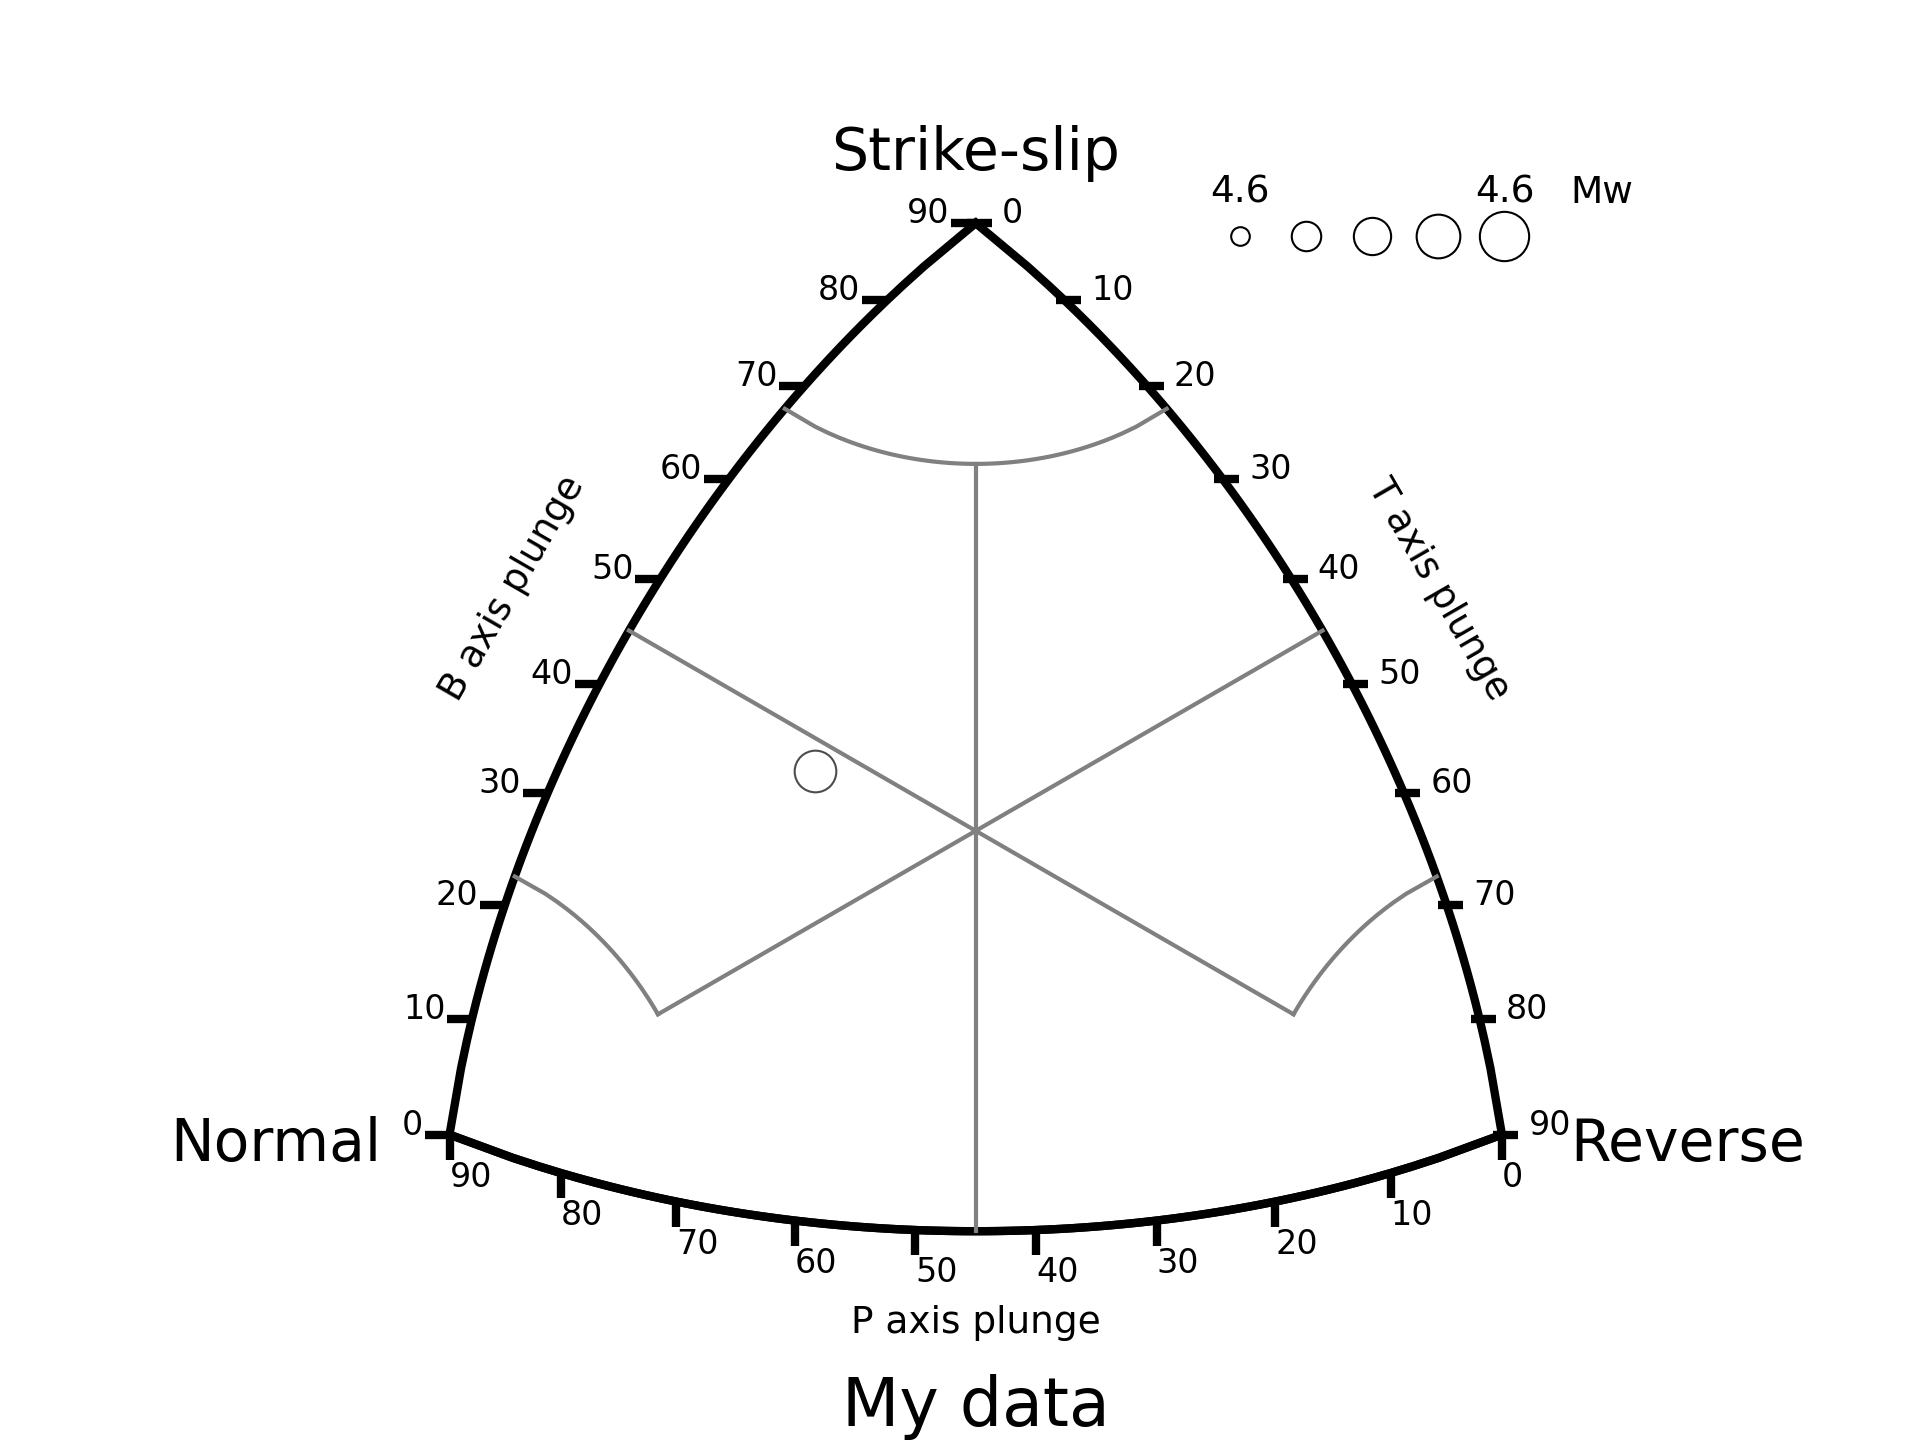
\includegraphics[width=0.55\textwidth]{figures/example_single_event.png}
\caption{Plot result from the command \texttt{echo -2.54 37.09 12 -3.4669 -2.0652 5.5321 6.2368 -1.8004 -5.1775 22 X Y ID | FMC.py -p ``My data.png''}}
\label{fig:example_single_event}
\end{figure}

\textbf{Plotting data from input file, shading the symbols with a parameter and plotting gridlines}

Command:

\begin{lstlisting}[language=bash]
FMC.py -p 'Japan data.png' jap_select.dat -pc dep -pg 10 -pt "Japan, Mw >= 7.2"
\end{lstlisting}

\begin{figure}[H]
\centering
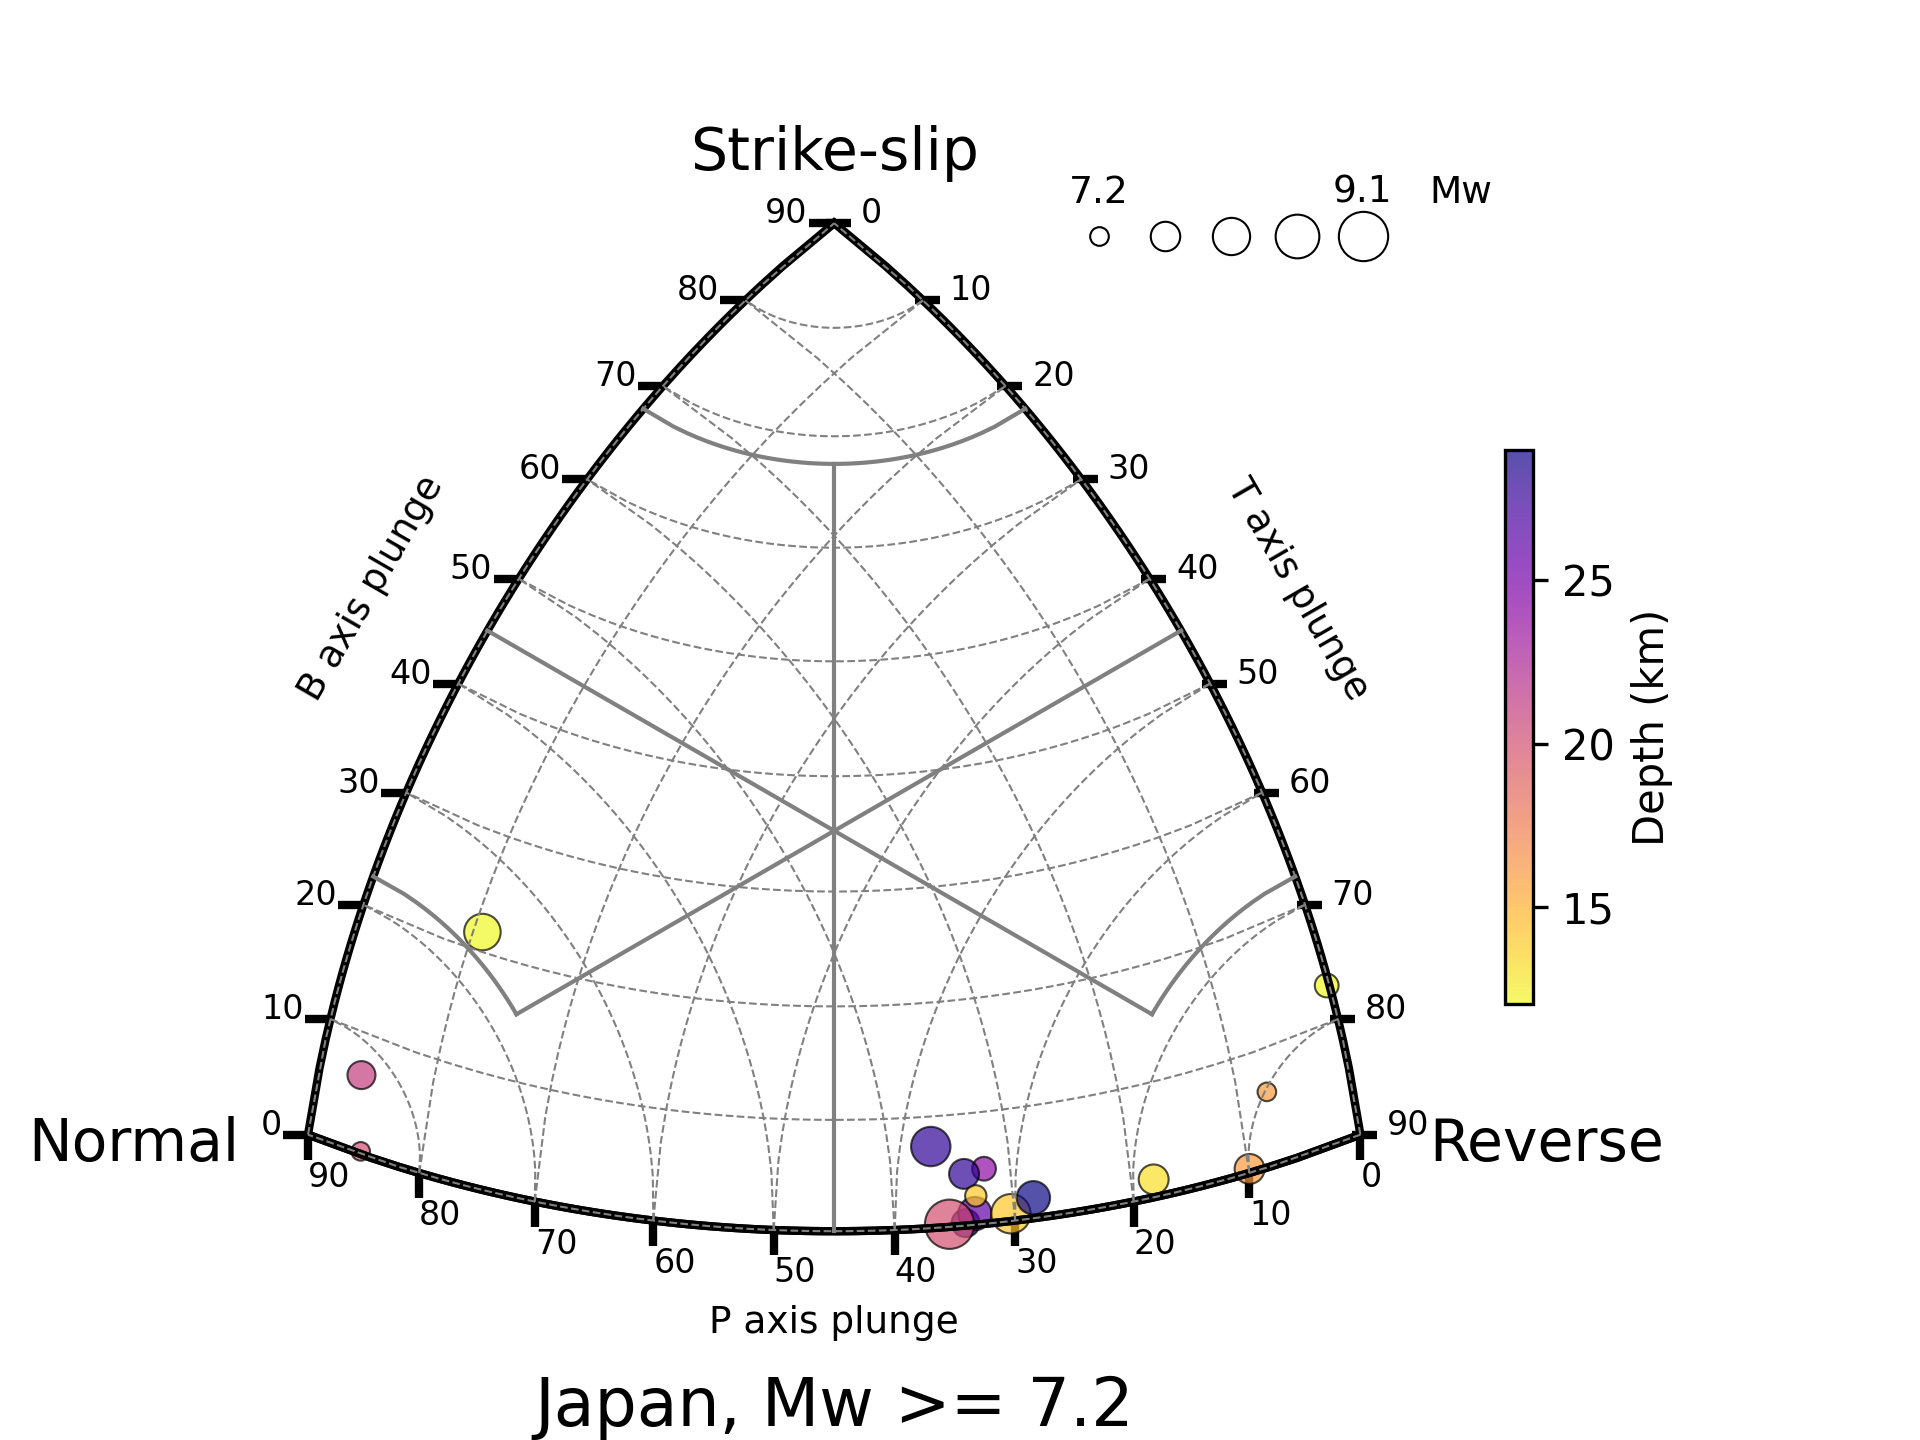
\includegraphics[width=0.55\textwidth]{figures/example_depth_grid.png}
\caption{Plot result from the command \texttt{FMC.py -p 'Japan data.png' jap\_select.dat -pc dep -pg 10 -pt ``Japan, Mw >= 7.2''}}
\label{fig:example_depth_grid}
\end{figure}

\textbf{Plotting data from input file shading and annotating the symbols}

Command:

\begin{lstlisting}[language=bash]
FMC.py jap_select.dat -p 'Japan labels.png' -pc dep -pa Mw -pt "Japan, Mw >= 7.2"
\end{lstlisting}

\begin{figure}[H]
\centering
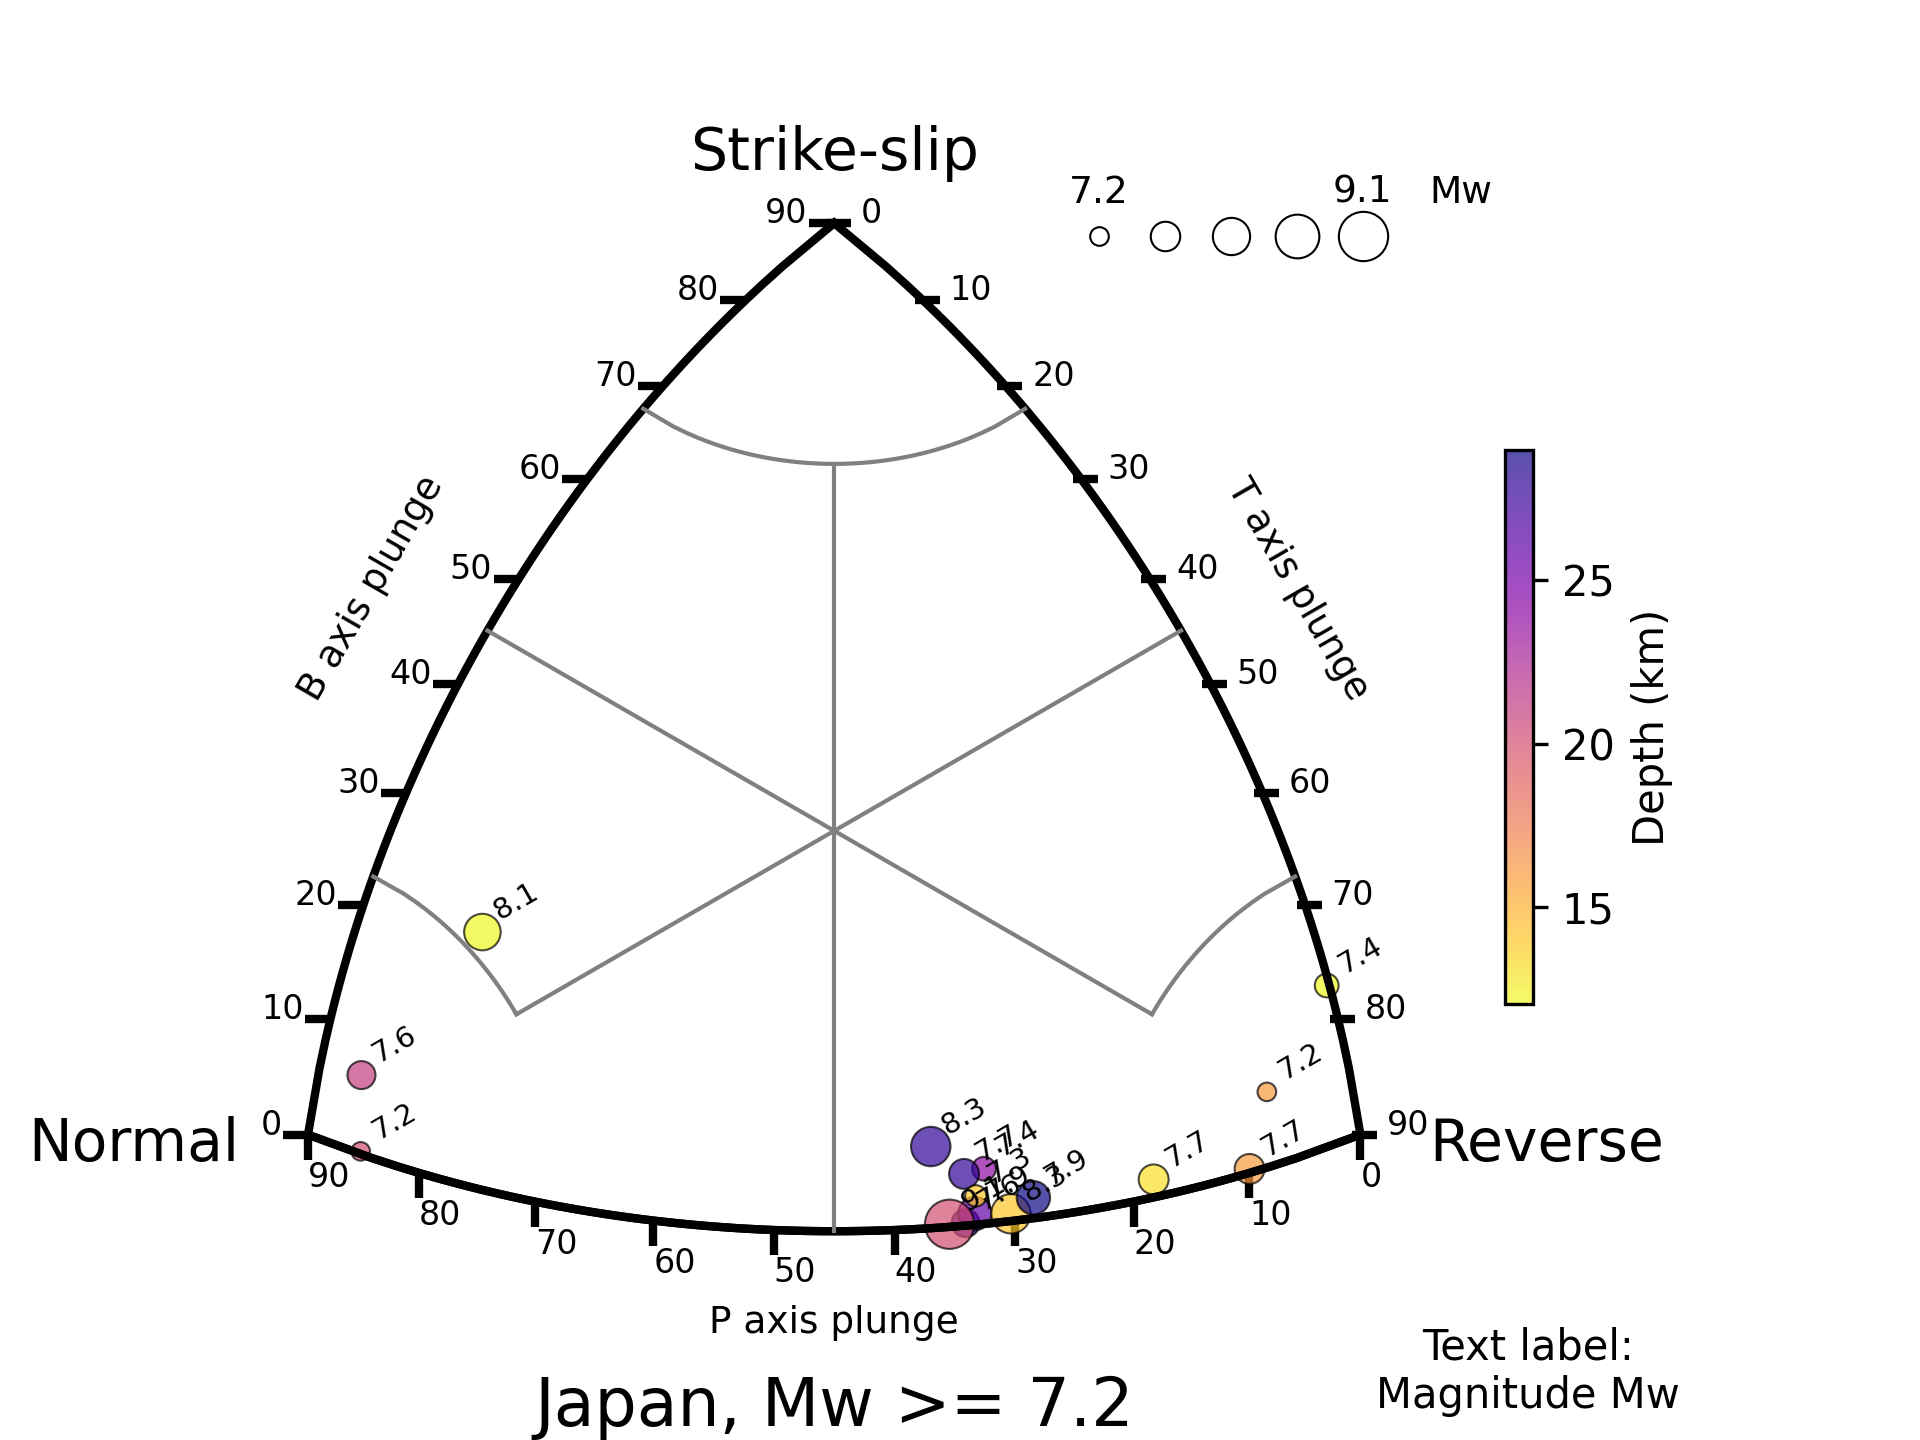
\includegraphics[width=0.55\textwidth]{figures/example_annotated.png}
\caption{Plot result from the command \texttt{FMC.py jap\_select.dat -p 'Japan labels.png' -pc dep -pa Mw -pt ``Japan, Mw >= 7.2''}}
\label{fig:example_annotated}
\end{figure}

\textbf{Plotting the source-type diagram}

Command:

\begin{lstlisting}[language=bash]
FMC.py jap_select.dat -pd 'Japan source type.png' -pc fclvd -pt "Japan, source type"
\end{lstlisting}

\begin{figure}[H]
\centering
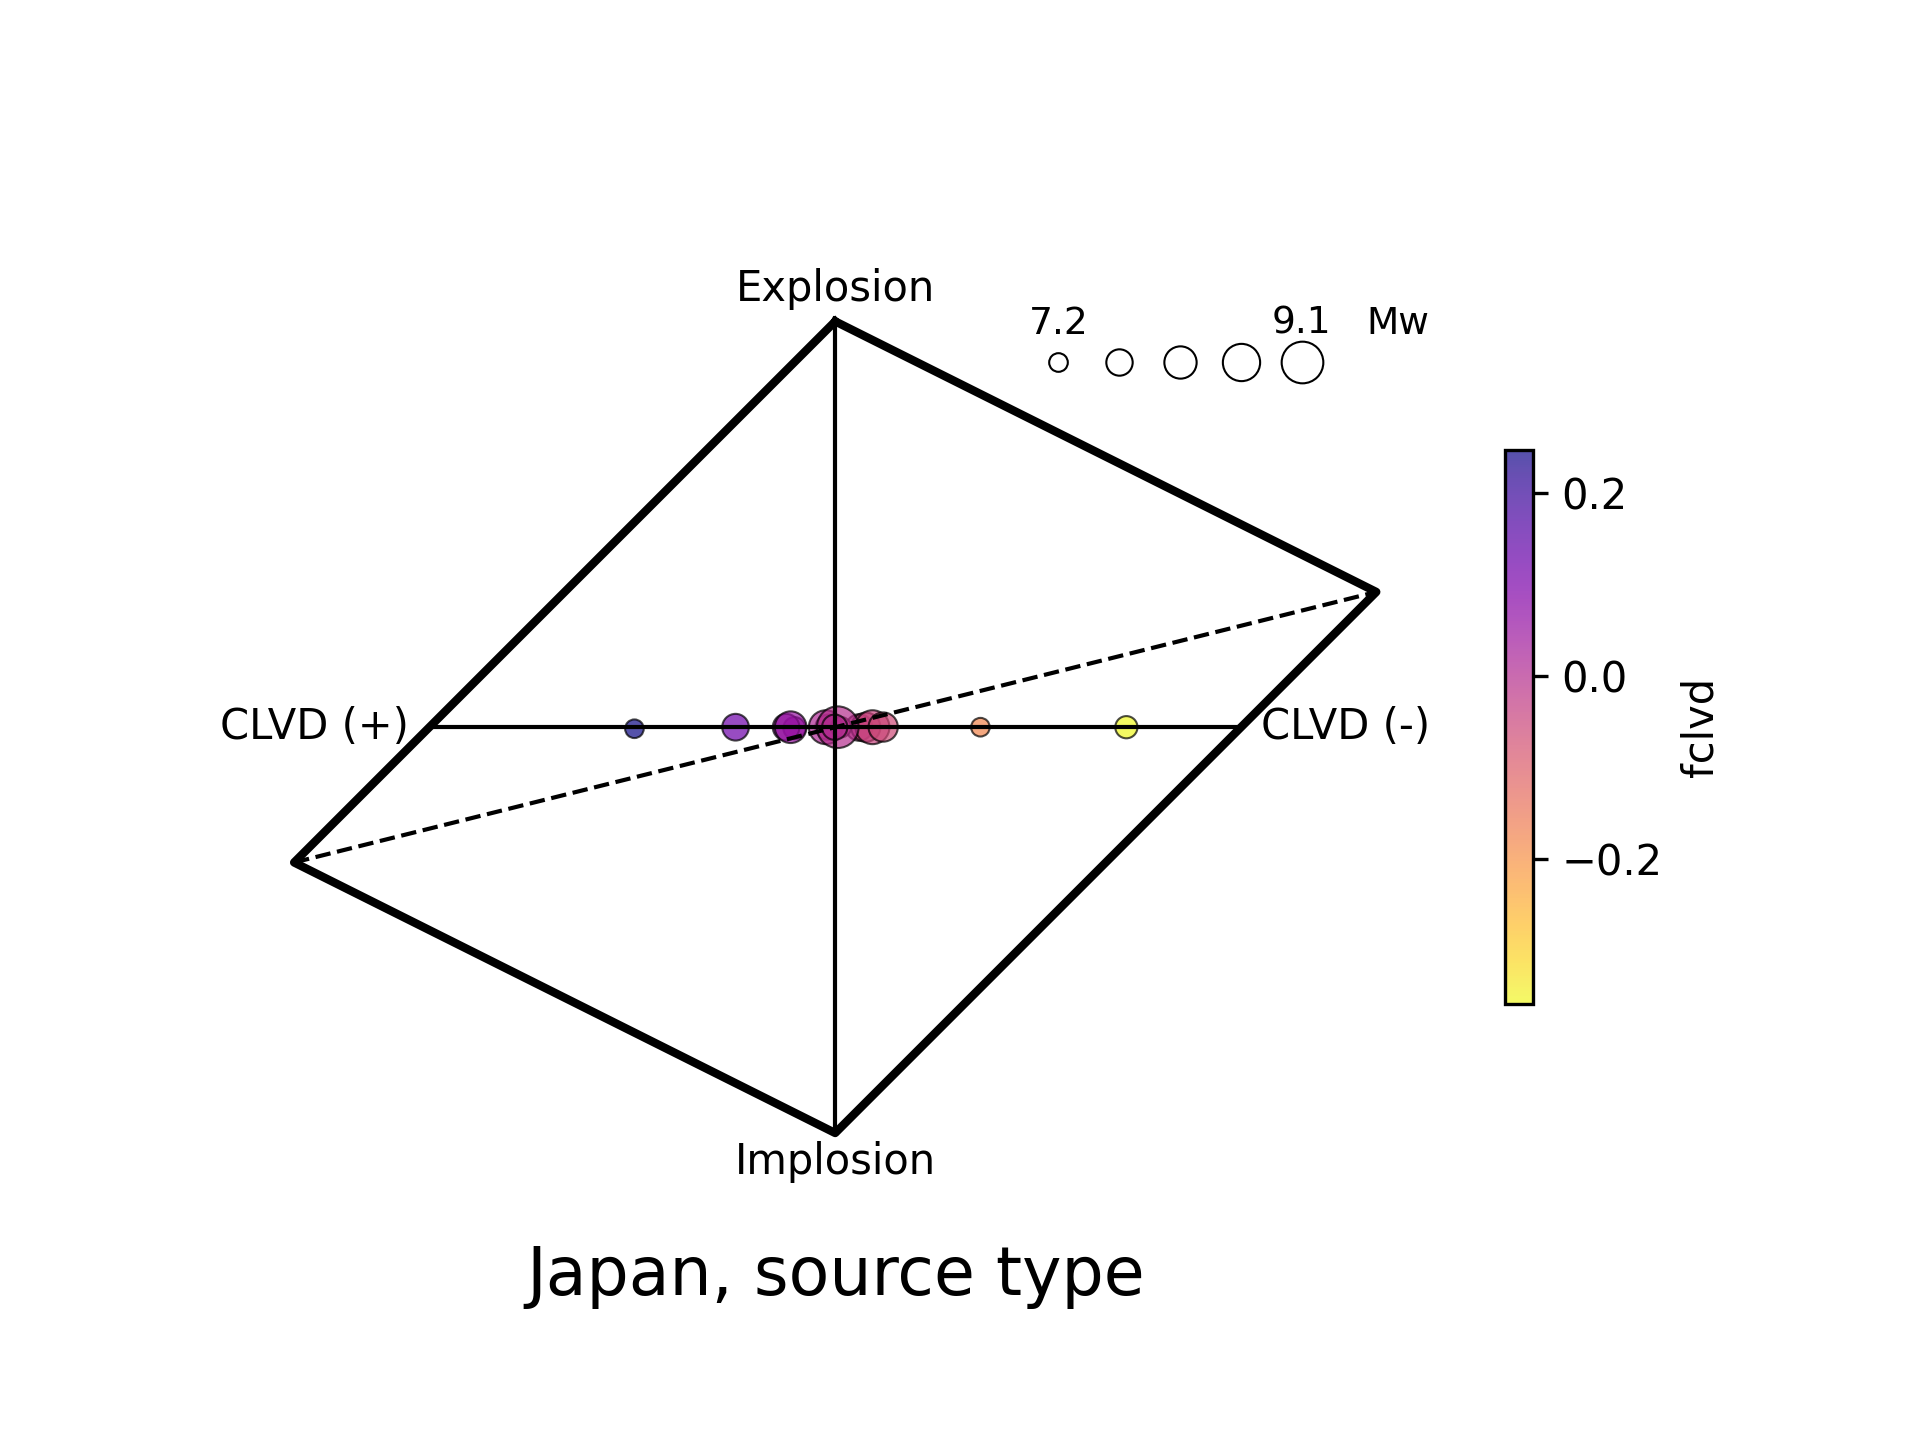
\includegraphics[width=0.60\textwidth]{figures/example_hudson.png}
\caption{Plot result from the command \texttt{FMC.py jap\_select.dat -pd 'Japan source type.png' -pc fclvd -pt ``Japan, source type''}. The Global CMT solutions are deviatoric, so all the events lie on the horizontal axis. Symbols are coloured by \texttt{fclvd}: positive values (purple, tension-dominated CLVD) plot on the left and negative values (yellow) on the right (section~\ref{sec:parameters-computed-by-fmc}).}
\label{fig:example_hudson}
\end{figure}

\textbf{Plotting P and T axes from fault-slip analysis}

Command:

\begin{lstlisting}[language=bash]
FMC.py -i PT pt_example.dat -p pt_axes.png -pc data1 -pt "Strain axes from fault-slip data"
\end{lstlisting}

\begin{figure}[H]
\centering
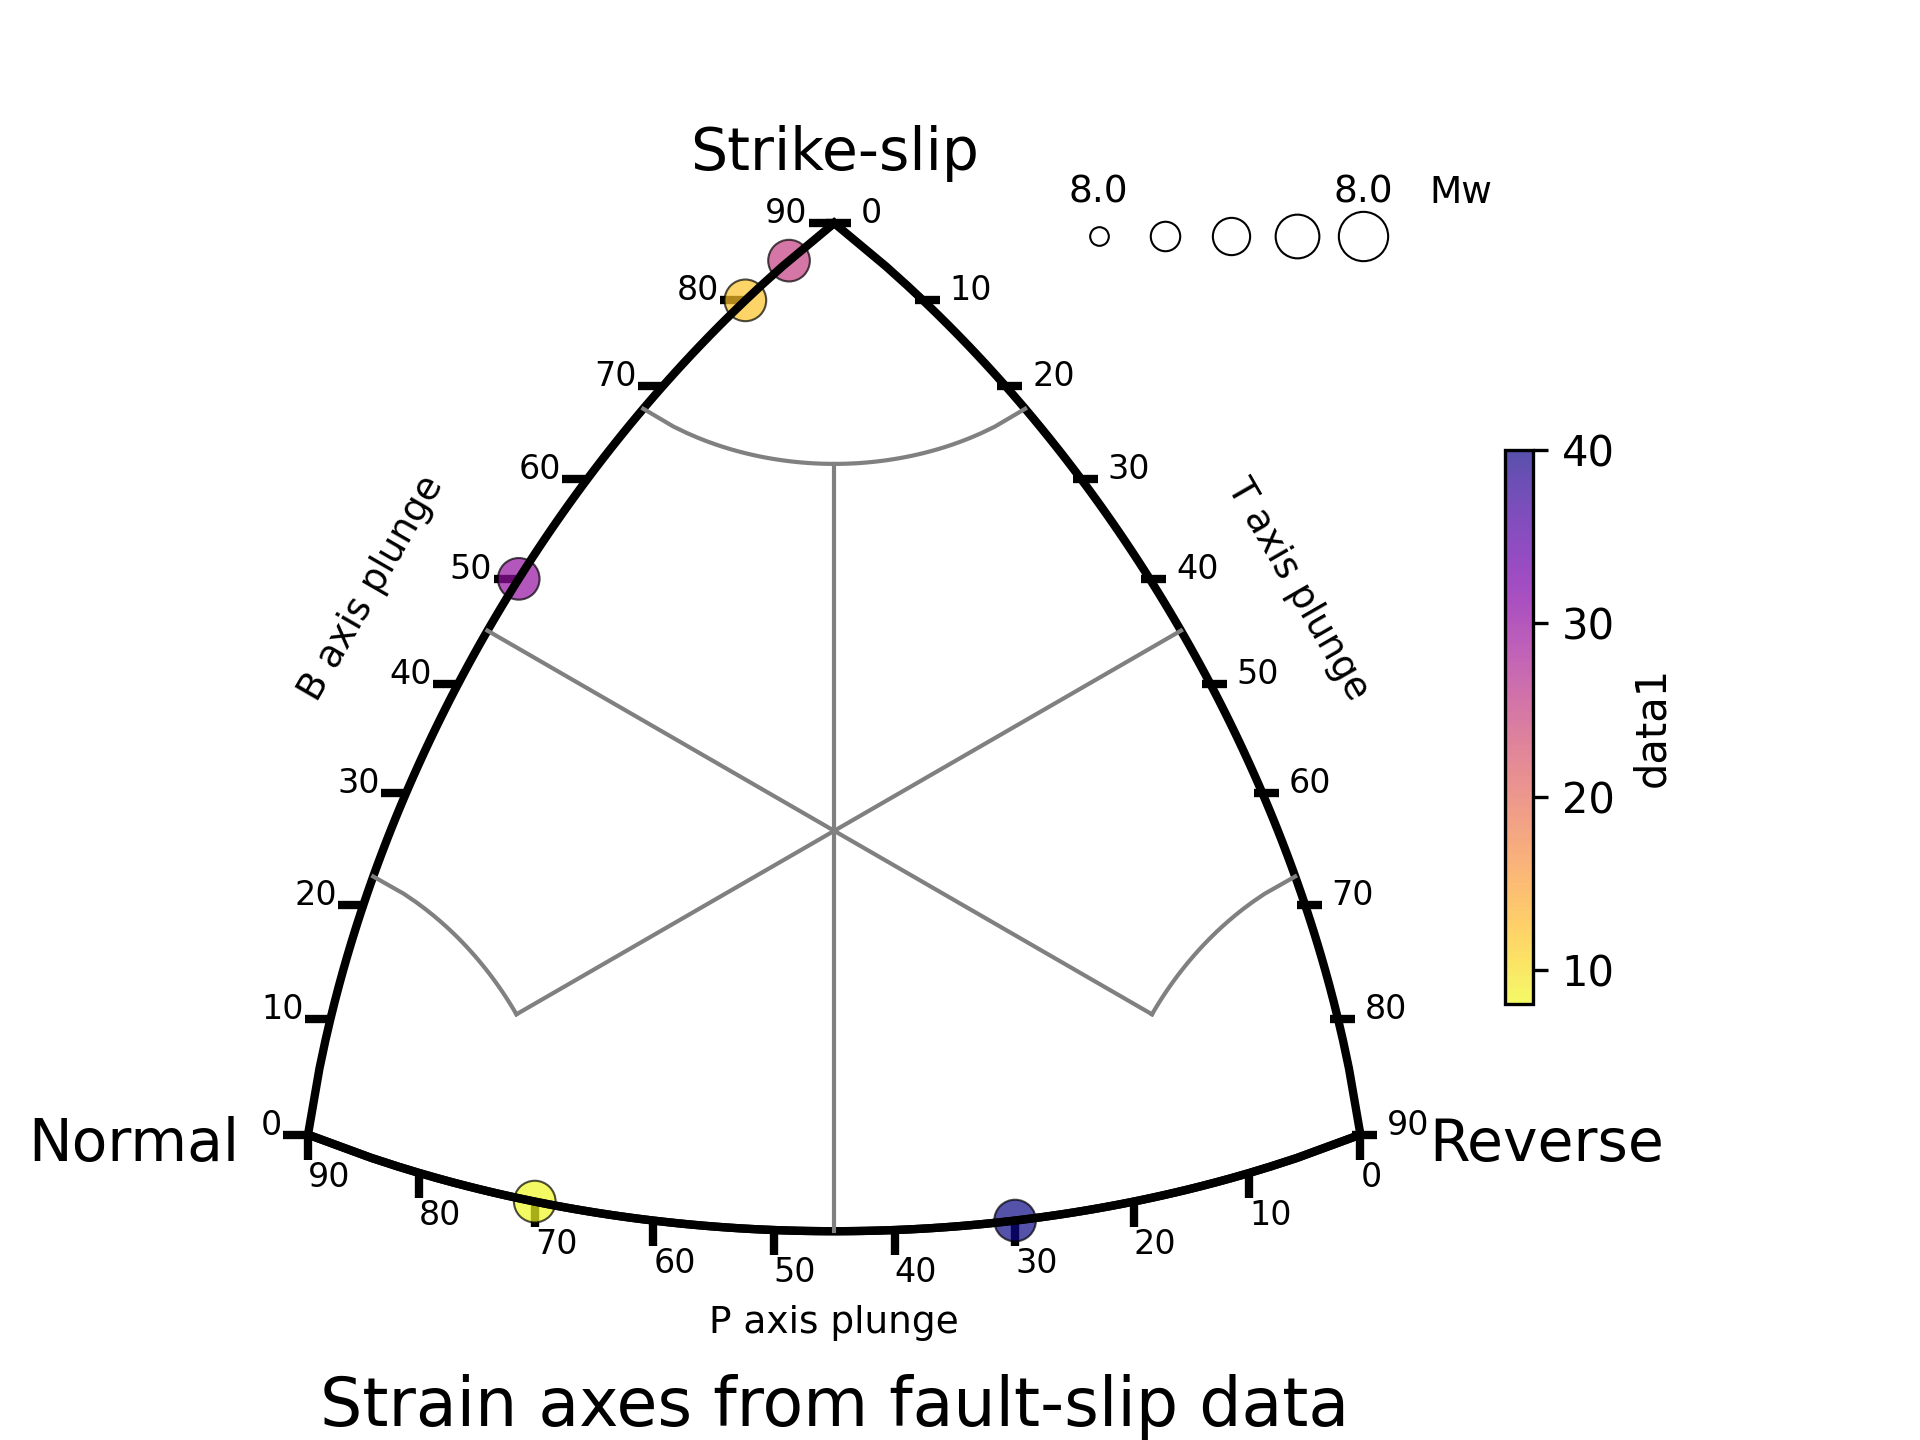
\includegraphics[width=0.55\textwidth]{figures/example_pt_input.png}
\caption{Plot result from the command \texttt{FMC.py -i PT pt\_example.dat -p pt\_axes.png -pc data1 -pt ``Strain axes from fault-slip data''}. All symbols have the same size because this format has no magnitude information.}
\label{fig:example_pt_input}
\end{figure}

\textbf{Plotting data from input file and piping to psmeca}

Command:

\begin{lstlisting}[language=bash]
FMC.py jap_select.dat | gmt psmeca -R125/170/30/60 -JM8c -Ba10f2WESN -Sm0.4c+f0 -Gred > CMT_map.ps
\end{lstlisting}

\begin{figure}[H]
\centering
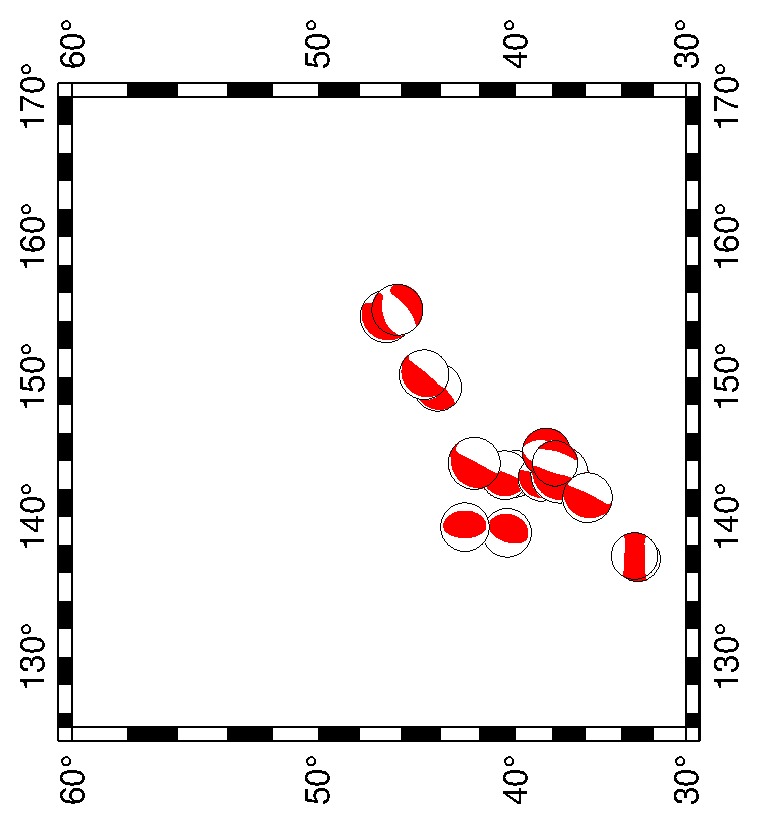
\includegraphics[width=0.45\textwidth, angle=-90]{figures/example_gmt_psmeca.png}
\caption{Map generated with \texttt{psmeca} (\texttt{GMT}) from the \texttt{FMC} output.}
\label{fig:example_gmt_psmeca}
\end{figure}

\subsection{Clustering}
\label{sec:clustering}

\texttt{FMC} implements the hierarchical agglomerative clustering
algorithms from SciPy (scipy.cluster.hierarchy) in order to group
the data\footnote{The details on the clustering algorithms shown in this section are
taken from the \href{https://docs.scipy.org/doc/scipy/reference/cluster.hierarchy.html\#module-scipy.cluster.hierarchy}{SciPy documentation}.}. The advantages of this algorithms are its versatility, as the
user can choose between a number of metrics and grouping methods,
its capacity to automatically select a minimum number of clusters
without an a priori estimation, and its potential to work with different
parameters with different scales and with strong different populations
in clusters.

The parameters for the clustering are passed by several optional flags.
If any of the following flags is given in the command line \texttt{FMC}
will perform the clustering analysis using some default options if
needed. When a clustering analysis is done, by default \texttt{FMC}
will shade the symbols in the diagram using the cluster number, unless
a different parameter is stated with \texttt{-pc} flag. The cluster number of each event is added as a last column (\texttt{Cluster\_ID}) to the output.
\begin{description}
\item[\texttt{-cm}] Method to be used in the clustering analysis. The
options are:

\begin{description}
\item[single] single/min/nearest 
\[
d(u,v)=\min(dist(u\left[i\right],v\left[j\right]))
\]
\item[complete] complete/max/farthest point 
\[
d(u,v)=\max(dist(u\left[i\right],v\left[j\right]))
\]
\item[average] average/UPGMA
\[
d(u,v)=\sum_{ij}\frac{d(u\left[i\right],v\left[j\right])}{(\left|u\right|*\left|v\right|)}
\]
\item[weighted] weighted/WPGMA
\[
d(u,v)=(dist(s,v)+dist(t,v))/2
\]
\item[centroid] centroid/UPGMC {[}default{]}
\[
dist(s,t)=\left\Vert c_{s}-c_{t}\right\Vert _{2}
\]
where $c_{s}$ and $c_{t}$ are the centroids of clusters $s$ and
$t$, respectively. When two clusters $s$ and $t$ are combined into
a new cluster $u$, the new centroid is computed over all the original
objects in clusters $s$ and $t$. The distance then becomes the Euclidean
distance between the centroid of $u$ and the centroid of a remaining
cluster $v$ in the forest.
\item[median] median/WPGMC, assigns $d(s,t)$ like the centroid method.
When two clusters $s$ and $t$ are combined into a new cluster $u$,
the average of centroids $s$ and $t$ give the new centroid.
\item[ward] Ward variance minimization algorithm.
\[
d(u,v)=\sqrt{\frac{\left|v\right|+\left|s\right|}{T}d(v,s)^{2}+\frac{\left|v\right|+\left|t\right|}{T}d(v,t)^{2}-\frac{\left|v\right|}{T}d(s,t)^{2}}
\]
where $u$ is the newly joined cluster consisting of clusters $s$
and $t$, $v$ is an unused cluster in the forest,$T=\left|v\right|+\left|s\right|+\left|t\right|$,
and $\left|*\right|$ is the cardinality of its argument.
\end{description}
Methods ``centroid'', ``median'' and ``ward'' are correctly
defined only if Euclidean pairwise metric is used. Since \texttt{centroid} is the default method, any other metric given with \texttt{-ce} must be combined with \texttt{-cm single}, \texttt{complete}, \texttt{average} or \texttt{weighted}; otherwise \texttt{FMC} stops with an error message.
\item[\texttt{-ce}] Metric used to measure distances between events
parameters. These metrics work with non-Boolean vectors. By default
\texttt{FMC} uses euclidean distance.

\begin{description}
\item[braycurtis] The Bray-Curtis distance between two points $u$ and
$v$ is 
\[
d(u,v)=\frac{\sum_{i}\left|u_{i}-v_{i}\right|}{\sum_{i}\left|u_{i}+v_{i}\right|}
\]
\item[canberra] The Canberra distance between two points $u$ and $v$
is
\[
d(u,v)=\underset{i}{\sum}\frac{\left|u_{i}-v_{i}\right|}{\left|u_{i}\right|+\left|v_{i}\right|}
\]
\item[chebyshev] The Chebyshev distance between two n-vectors $u$ and
$v$ is the maximum norm-1 distance between their respective elements.
More precisely, the distance is given by
\[
d(u,v)=\underset{i}{\max}\left|u_{i}-v_{i}\right|
\]
\item[cityblock] City block or Manhattan distance between the points.
\item[correlation] Correlation distance between vectors $u$ and $v$.
This is
\[
1-\frac{(u-\bar{u})\cdot (v-\bar{v})}{\left\Vert (u-\bar{u})\right\Vert _{2}\left\Vert (v-\bar{v})\right\Vert _{2}}
\]
\item[cosine] Cosine distance between vectors $u$ and $v$, 
\[
1-\frac{u\cdot v}{\left\Vert u\right\Vert _{2}\left\Vert v\right\Vert _{2}}
\]
\item[euclidean] Distance between m points using Euclidean distance
(2-norm). {[}Default{]}
\item[hamming] Normalized Hamming distance, or the proportion of those
vector elements between two n-vectors $u$ and $v$ which disagree.
\item[jaccard] Jaccard distance between the points. Given two vectors,
$u$ and $v$, the Jaccard distance is the proportion of those elements
$u[i]$ and $v[i]$ that disagree.
\item[mahalanobis] The Mahalanobis distance between two points $u$
and $v$ is
\[
\sqrt{(u-v)(1/V)(u-v)^{T}}
\]
where $1/V$ is the inverse covariance matrix.
\item[minkowski] Distances using the Minkowski distance $\left\Vert u-v\right\Vert _{p}$
(p-norm) where $p\geq1$.
\item[seuclidean] Standardized Euclidean distance. The standardized
Euclidean distance between two n-vectors $u$ and $v$ is
\[
\sqrt{\sum\left(u_{i}-v_{i}\right)^{2}\div V\left[x_{i}\right]}
\]
$V$ is the variance vector; $V[i]$ is the variance computed over
all the i’th components of the points. It is automatically computed.
\item[sqeuclidean] Squared Euclidean distance $\left\Vert u-v\right\Vert _{2}^{2}$
between the vectors.
\end{description}
\item[\texttt{-cn}] A priori number of clusters to obtain. If zero or
non-present the number of clusters is automatically computed with an elbow criterion on the dendrogram: the merging distances are taken from the last merge to the first and the number of clusters is set where their second difference is largest (the minimum is two clusters).
\item[\texttt{-ci}] Parameters used to perform the cluster analysis.
By default \texttt{FMC} uses the position on the Kaverina diagram,
which is a proxy for the principal moment tensor axes plunges. If
the parameters given are not in the same physical magnitude and unit
the euclidean distance is not appropriate and a different metric should
be used. In these cases the Mahalanobis distance is a good choice,
as is equivalent to the Euclidean distance in the transformed space,
using the covariance matrix of each parameter. Angular parameters such as strikes and trends are circular (0° and 360° are the same direction), which is not taken into account by any of these metrics.

The parameters must be given with its corresponding internal name
as listed in section \ref{sec:output}.
\end{description}

\subsubsection{Examples of use}

\textbf{Automatic clustering using the position in the Kaverina diagram (default)}

Command:

\begin{lstlisting}[language=bash]
FMC.py -p 'Japan clusters.png' jap_select.dat -cn 0 -pt "Japan, automatic clustering"
\end{lstlisting}

\begin{figure}[H]
\centering
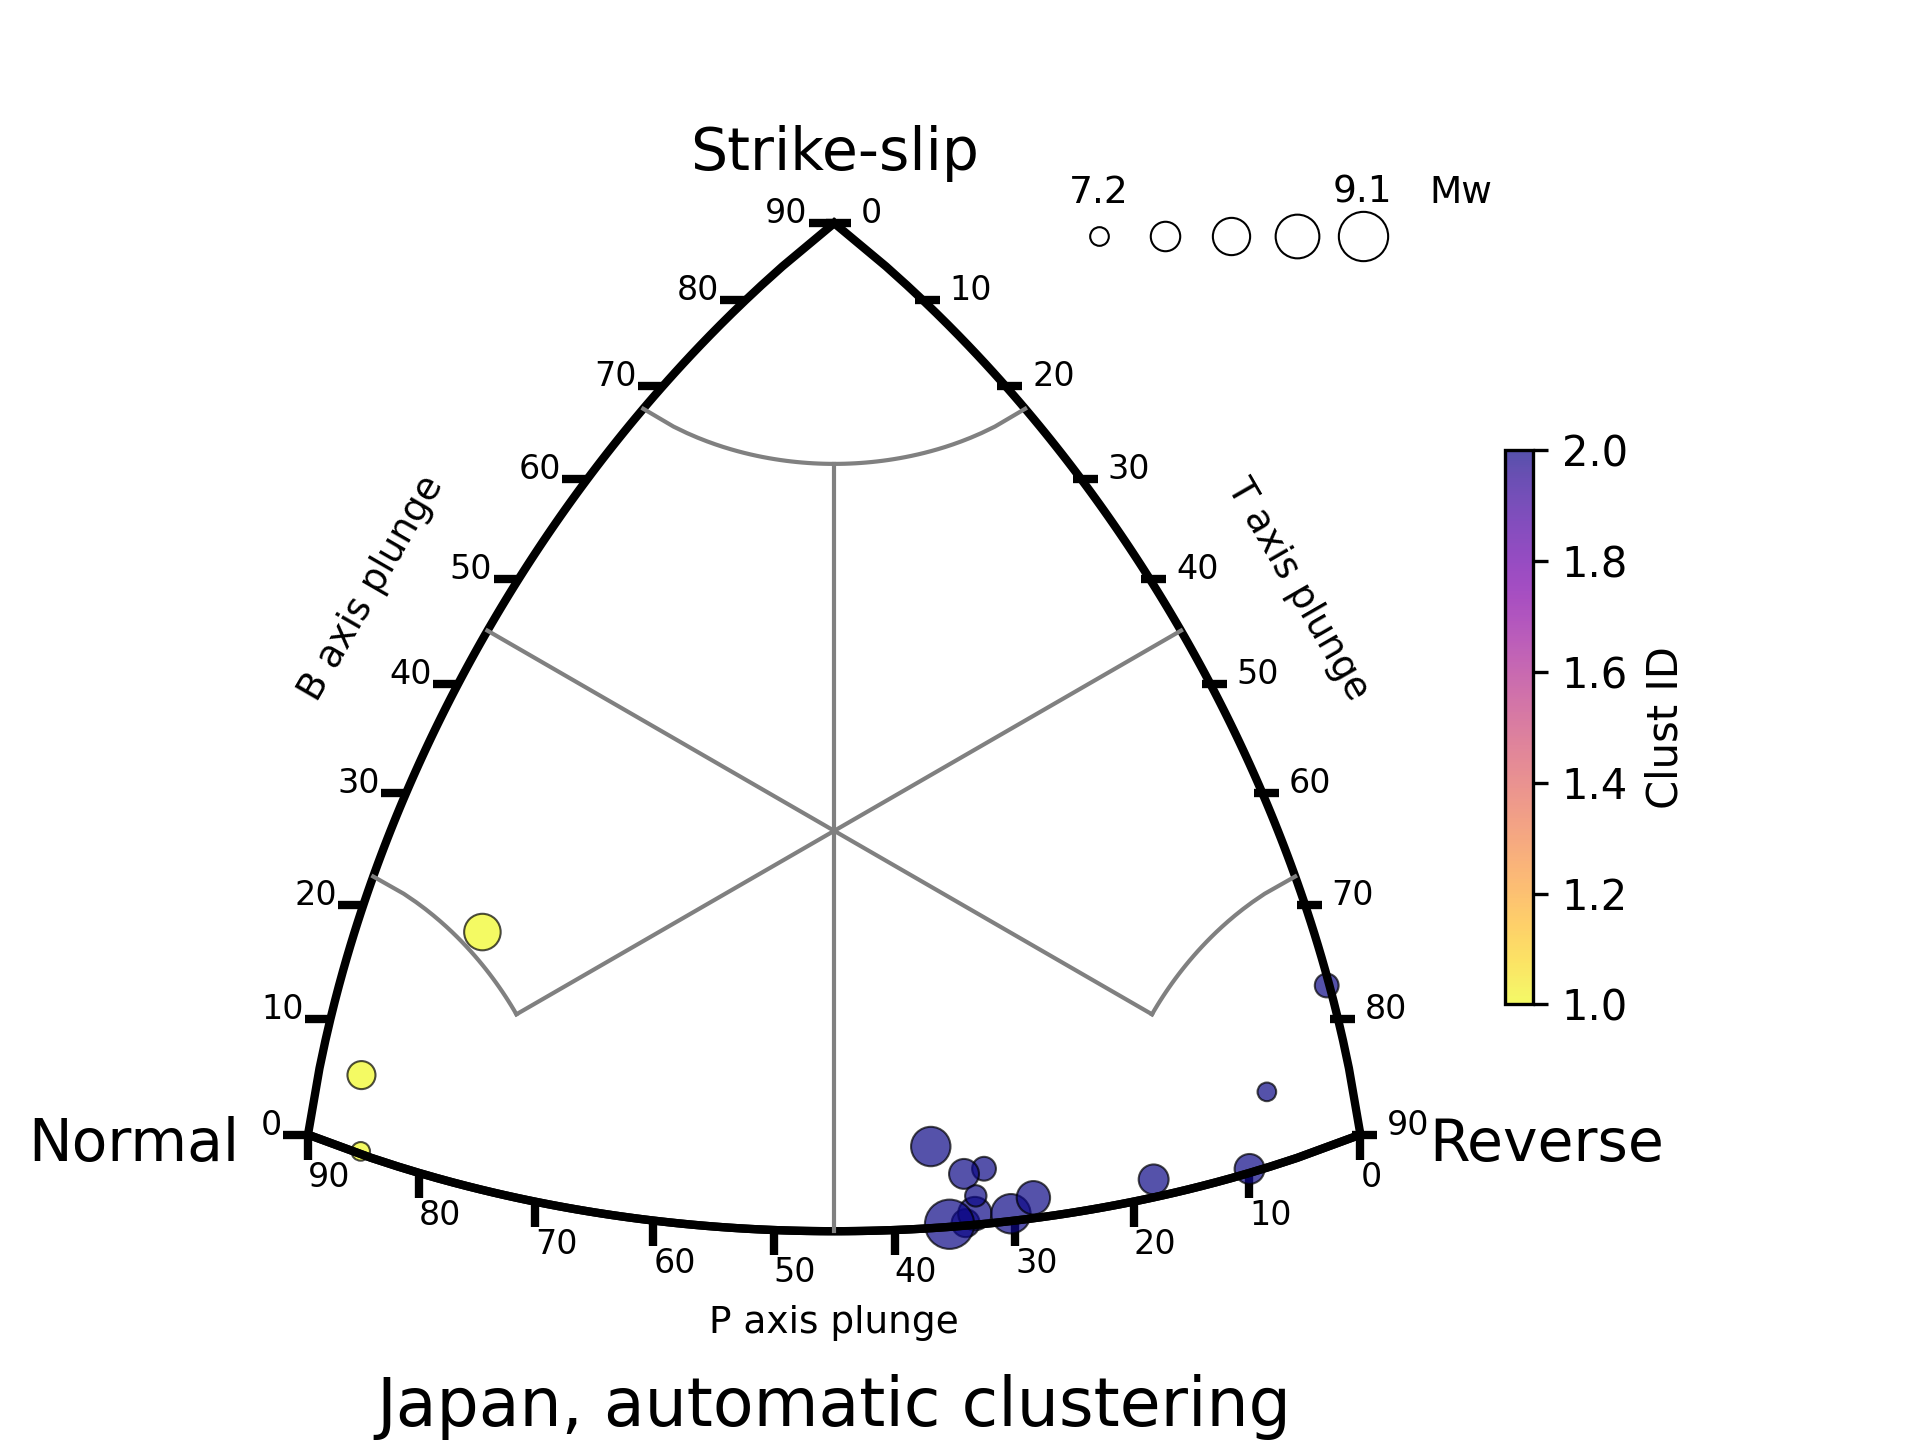
\includegraphics[width=0.55\textwidth]{figures/example_clusters_auto.png}
\caption{Plot result from the command \texttt{FMC.py -p 'Japan clusters.png' jap\_select.dat -cn 0 -pt ``Japan, automatic clustering''}}
\label{fig:example_clusters_auto}
\end{figure}

The output contains the cluster of each event in the last column:

\begin{lstlisting}
#ID Magnitude_Mw rupture_type Cluster_ID
032378C 7.6 R 2
052683A 7.7 R 2
110189E 7.4 R 2
071293B 7.7 R 2
\end{lstlisting}

\textbf{Clustering using the epicentral location}

Command:

\begin{lstlisting}[language=bash]
FMC.py jap_select.dat -cn 3 -ci lon,lat > clusters.dat
\end{lstlisting}

\begin{figure}[H]
\centering
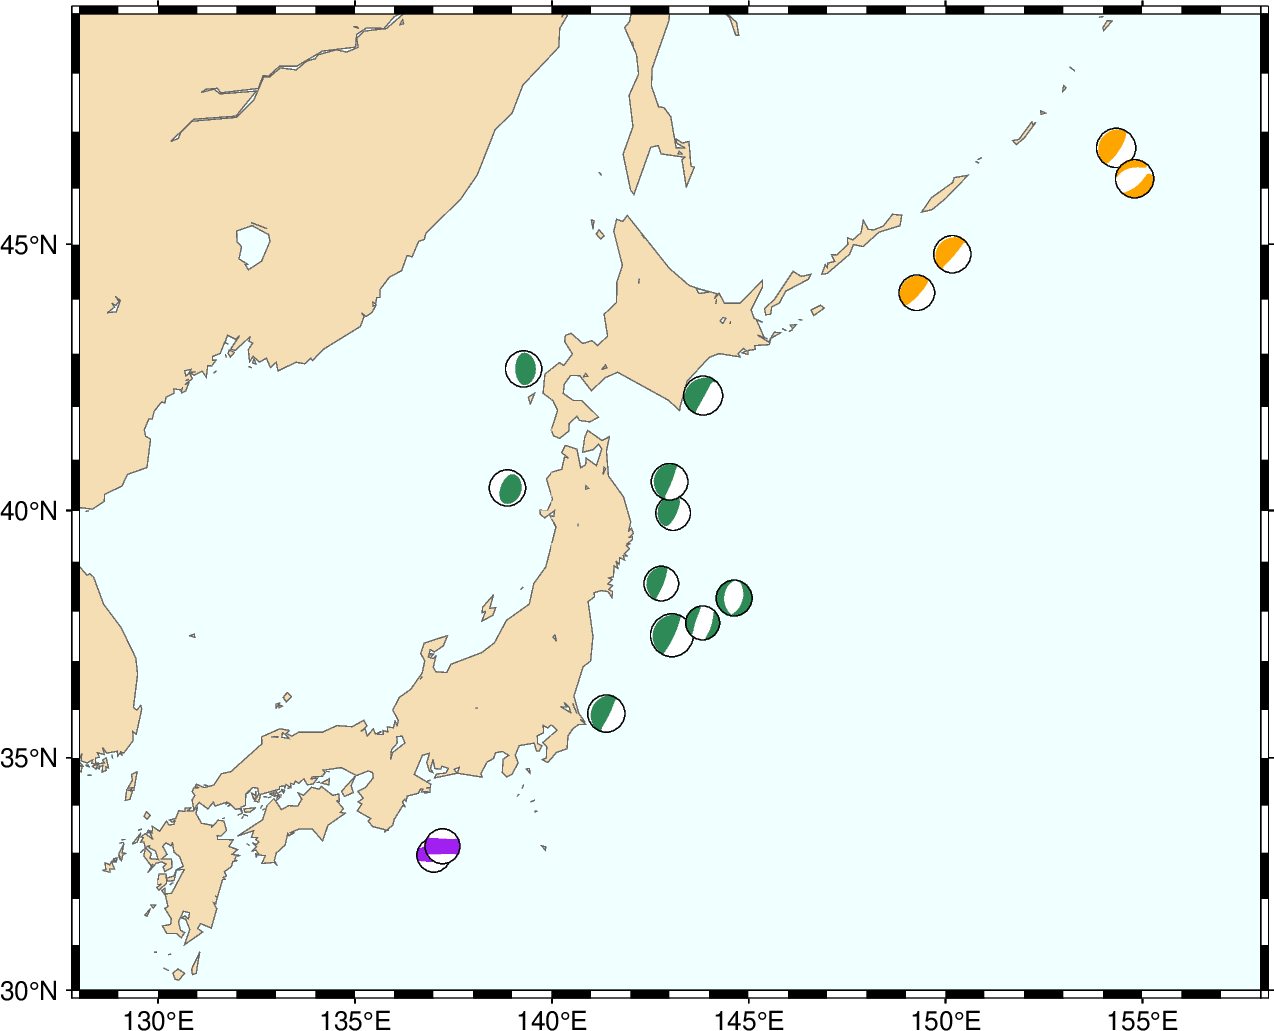
\includegraphics[width=0.60\textwidth]{figures/example_gmt_spatial_clusters.png}
\caption{Plotting with \texttt{GMT} of the clusters obtained with the command \texttt{FMC.py jap\_select.dat -cn 3 -ci lon,lat} (see section~\ref{sec:working-with-gmt}).}
\label{fig:example_gmt_spatial_clusters}
\end{figure}

\textbf{Clustering using Mahalanobis metric and complete grouping with the slip and plunge of the slip vector of nodal plane A}

Command:

\begin{lstlisting}[language=bash]
FMC.py -p 'Japan clusters plane A.png' jap_select.dat -cn 3 -ci slipA,plungA -cm complete -ce mahalanobis
\end{lstlisting}

\begin{figure}[H]
\centering
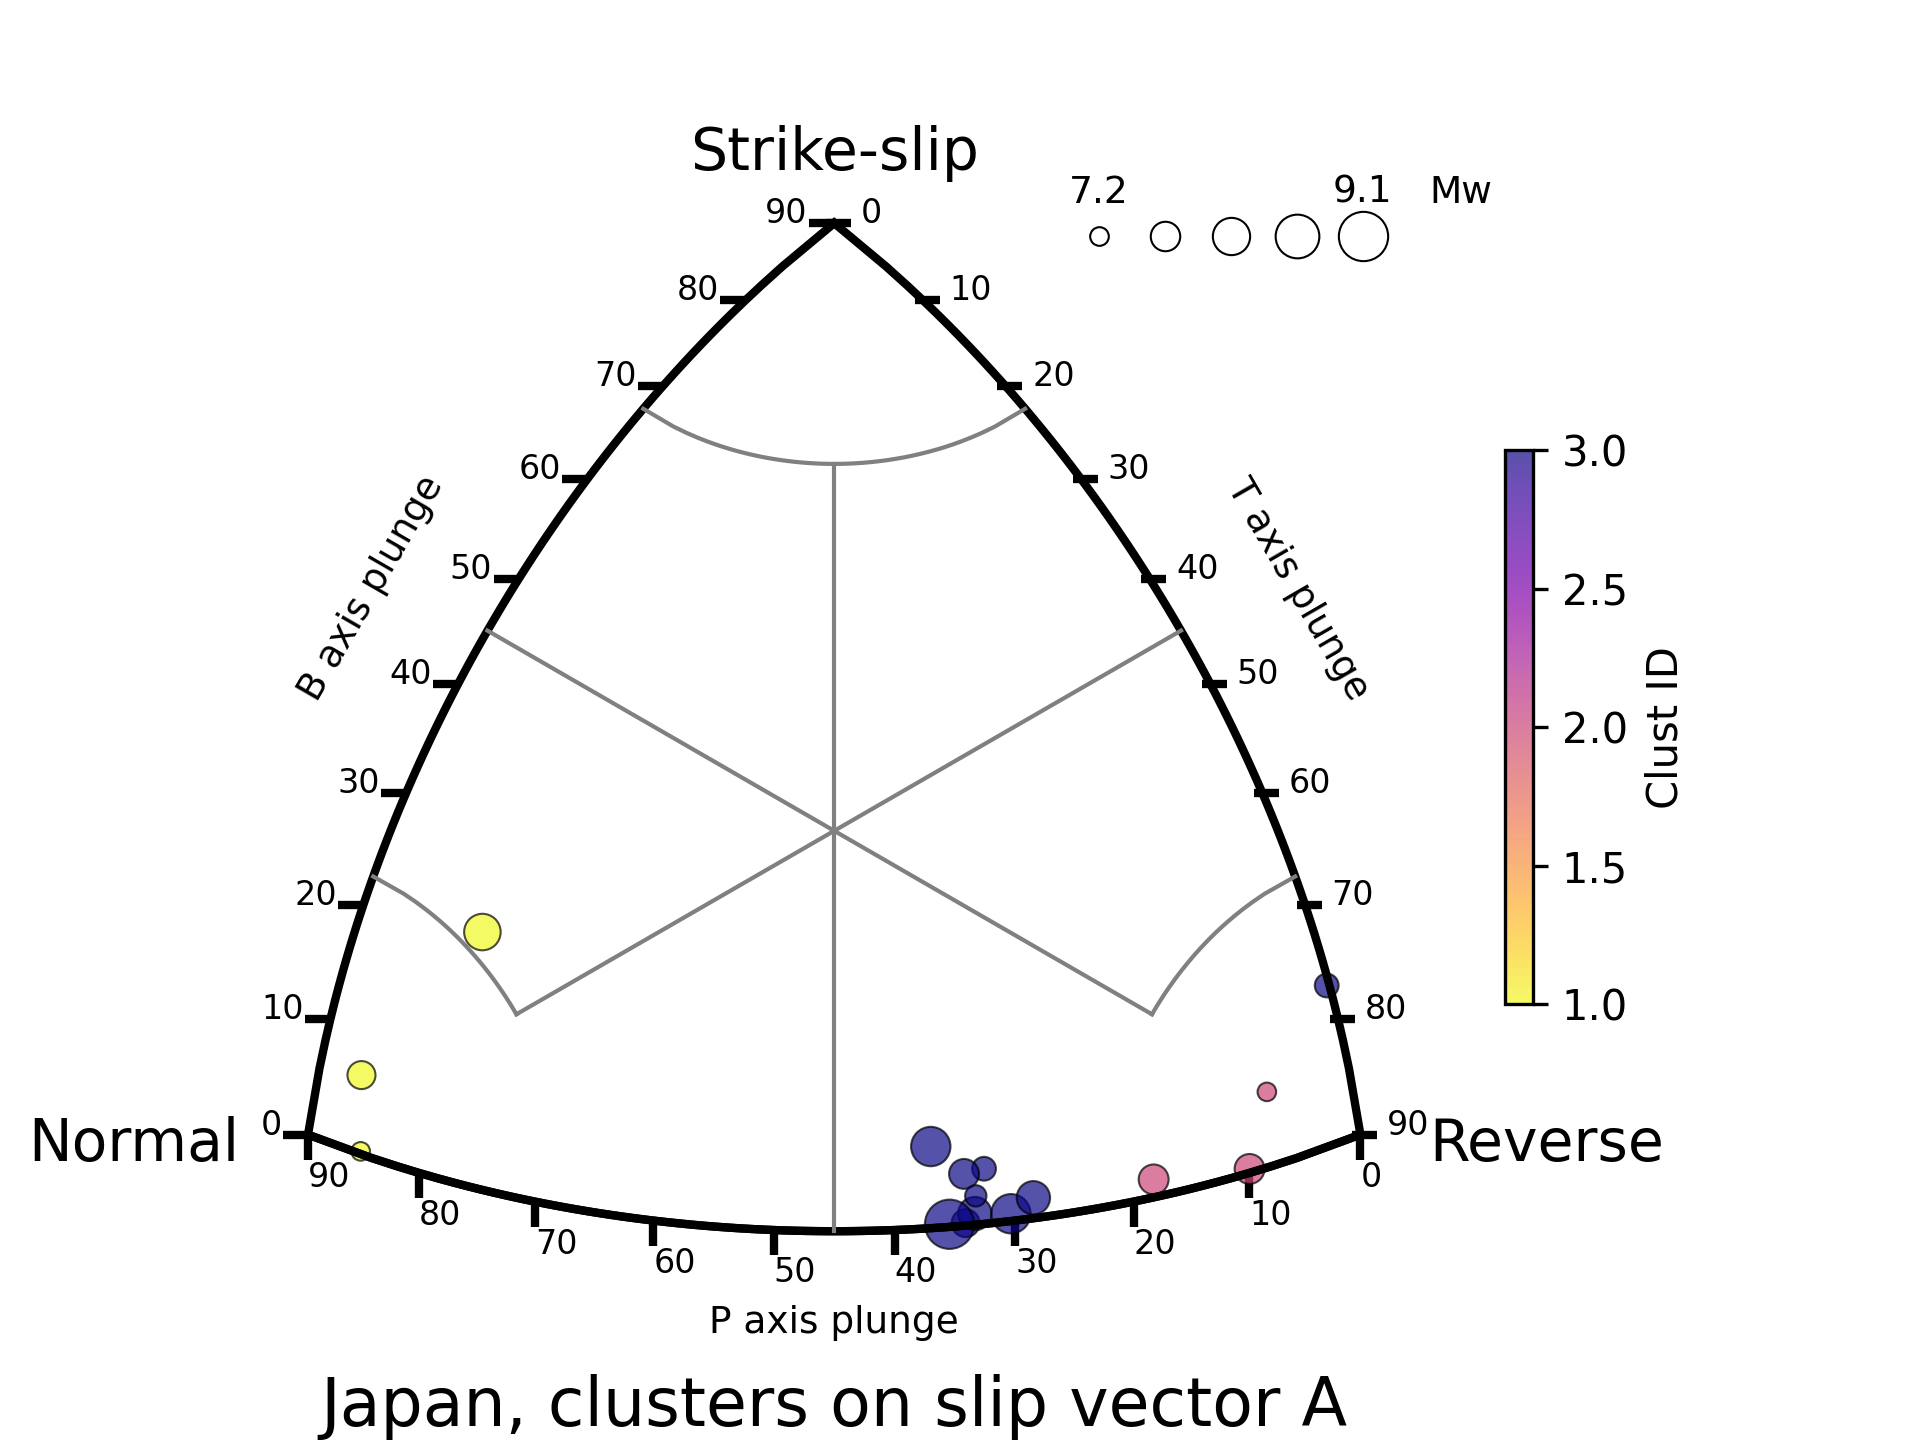
\includegraphics[width=0.55\textwidth]{figures/example_clusters_slip.png}
\caption{Plot result from the command \texttt{FMC.py -p 'Japan clusters plane A.png' jap\_select.dat -cn 3 -ci slipA,plungA -cm complete -ce mahalanobis}}
\label{fig:example_clusters_slip}
\end{figure}

\subsection{Working with GMT}
\label{sec:working-with-gmt}

The \texttt{CMT}, \texttt{P} and \texttt{AR} outputs can be read directly by the \texttt{GMT} module \texttt{meca} (\texttt{psmeca} in GMT 4 and 5), with the symbol options \texttt{-Sm}, \texttt{-Sc} and \texttt{-Sa} respectively. The header line starts with \texttt{\#} and is skipped by \texttt{GMT}. The last columns (\texttt{ID}, \texttt{rupture\_type} and, if present, \texttt{Cluster\_ID}) are read as the event label; add \texttt{+f0} to the symbol option to hide the labels.

\begin{lstlisting}[language=bash]
FMC.py jap_select.dat | gmt psmeca -R125/170/30/60 -JM8c -Ba10f2WESN -Sm0.4c > CMT_map.ps
FMC.py jap_select.dat | gmt meca -R128/158/30/49 -JM15c -Baf -Sm0.3c -png japan_map
\end{lstlisting}

The rupture type is written in column 14 of the \texttt{CMT} output, so the mechanisms can be coloured by tectonic regime with \texttt{awk}. Here \texttt{/\textasciicircum N/} selects the classes N and N-SS, \texttt{/\textasciicircum SS/} selects SS, SS-N and SS-R, and \texttt{/\textasciicircum R/} selects R and R-SS:

\begin{lstlisting}[language=bash]
gmt begin japan_rupture_type png
  gmt coast -R128/158/30/49 -JM15c -Baf -BWSne -Gwheat -Sazure -W0.25p,gray40
  FMC.py jap_select.dat | awk '$14 ~ /^N/'  | gmt meca -Sm0.3c+f0 -Gdodgerblue -W0.3p
  FMC.py jap_select.dat | awk '$14 ~ /^SS/' | gmt meca -Sm0.3c+f0 -Gforestgreen -W0.3p
  FMC.py jap_select.dat | awk '$14 ~ /^R/'  | gmt meca -Sm0.3c+f0 -Gred -W0.3p
gmt end show
\end{lstlisting}

\begin{figure}[H]
\centering
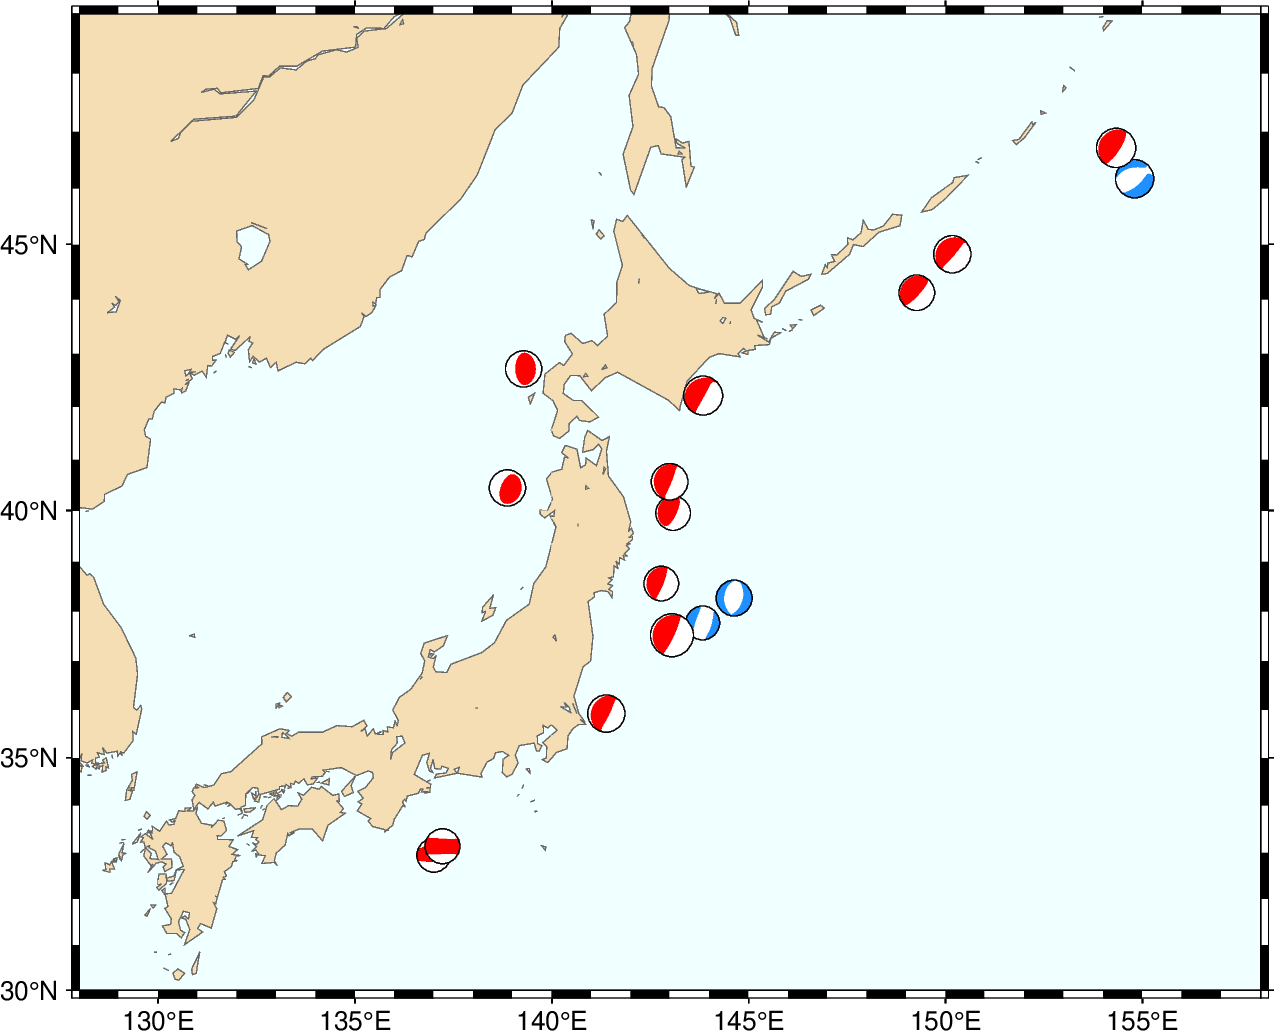
\includegraphics[width=0.60\textwidth]{figures/example_gmt_rupture_type.png}
\caption{GMT map of the test data coloured by regime: normal and normal -- strike-slip in blue, reverse in red.}
\label{fig:example_gmt_rupture_type}
\end{figure}

Similarly, the clusters can be mapped using the \texttt{Cluster\_ID} column (column 15 of the \texttt{CMT} output):

\begin{lstlisting}[language=bash]
FMC.py jap_select.dat -cn 3 -ci lon,lat > clusters.dat
gmt begin japan_spatial_clusters png
  gmt coast -R128/158/30/49 -JM15c -Baf -BWSne -Gwheat -Sazure -W0.25p,gray40
  awk '$15==1' clusters.dat | gmt meca -Sm0.3c+f0 -Gorange -W0.3p
  awk '$15==2' clusters.dat | gmt meca -Sm0.3c+f0 -Gpurple -W0.3p
  awk '$15==3' clusters.dat | gmt meca -Sm0.3c+f0 -Gseagreen -W0.3p
gmt end show
\end{lstlisting}

\subsection{Command-line reference}
\label{sec:command-line-reference}

\begin{lstlisting}
FMC.py [infile] [-i {CMT,AR,P,PT}] [-o {CMT,P,AR,K,ALL,CUSTOM}] [-of FIELDS]
       [-p PLOTFILE] [-pd PLOTFILE] [-pc PARAM] [-pa PARAM] [-pg SPACING] [-pt TITLE]
       [-cm METHOD] [-ce METRIC] [-cn N] [-ci FIELDS]
       [-v] [-helpFields] [-h]
\end{lstlisting}

\begin{longtable}{p{0.163\linewidth}p{0.631\linewidth}p{0.102\linewidth}}
\toprule
\textbf{Flag} & \textbf{Description} & \textbf{Section} \\
\midrule
\endhead
\texttt{infile} & Input file; if absent, FMC reads the standard input & \ref{sec:input} \\
\texttt{-i} & Input format: \texttt{CMT} (default), \texttt{AR}, \texttt{P}, \texttt{PT} & \ref{sec:input} \\
\texttt{-o} & Output format: \texttt{CMT} (default), \texttt{P}, \texttt{AR}, \texttt{K}, \texttt{ALL}, \texttt{CUSTOM} & \ref{sec:output} \\
\texttt{-of} & Comma-separated parameters for \texttt{-o\ CUSTOM} & \ref{sec:output} \\
\texttt{-p} & Classification diagram file & \ref{sec:plot} \\
\texttt{-pd} & Source-type diagram file & \ref{sec:plot} \\
\texttt{-pc} & Parameter used to colour the symbols & \ref{sec:plot} \\
\texttt{-pa} & Parameter used to label the symbols & \ref{sec:plot} \\
\texttt{-pg} & Gridline spacing in degrees & \ref{sec:plot} \\
\texttt{-pt} & Plot title & \ref{sec:plot} \\
\texttt{-cm} & Clustering linkage method & \ref{sec:clustering} \\
\texttt{-ce} & Clustering distance metric & \ref{sec:clustering} \\
\texttt{-cn} & Number of clusters (0: automatic) & \ref{sec:clustering} \\
\texttt{-ci} & Comma-separated clustering parameters & \ref{sec:clustering} \\
\texttt{-v} & Verbose: progress information on the standard error & --- \\
\texttt{-helpFields} & Lists the parameter names and exits & \ref{sec:output} \\
\texttt{-h} & Shows the help and exits & --- \\
\bottomrule
\end{longtable}

\subsection{Troubleshooting and known issues}
\label{sec:troubleshooting-and-known-issues}

\textbf{``ERROR - Incorrect number of columns''.} Each input format requires an exact number of
columns (13, 10, 14 or 10 for \texttt{CMT}, \texttt{AR}, \texttt{P} and \texttt{PT}). Check the
chosen \texttt{-i} format, remove extra columns (such as the \texttt{rupture\_type} column of a
previous FMC output) and make sure that event IDs contain no spaces.

\textbf{``ERROR - The clustering methods `centroid', `median' and `ward' only work with the
`euclidean' metric''.} A non-Euclidean metric was chosen with \texttt{-ce} while keeping the default
linkage method. Add \texttt{-cm\ single}, \texttt{complete}, \texttt{average} or \texttt{weighted},
or use \texttt{-ce\ euclidean}.

\textbf{``Warning, to fill the symbols a numeric value is needed''.} The parameter chosen with
\texttt{-pc} is not numeric (for example \texttt{clas} or alphanumeric event IDs); the symbols are
drawn in white.

\textbf{\texttt{BrokenPipeError} when piping into \texttt{head}.} Harmless: the output was
interrupted by the receiving program after it read what it needed.

\textbf{PT input gives unexpected planes.} The P and T axes must be orthogonal; FMC does not check
or correct this.

\textbf{Errors in versions before 1.9.1.} In FMC 1.9 and earlier, \texttt{-pa} fails with
\texttt{TypeError:\ only\ 0-dimensional\ arrays\ can\ be\ converted\ to\ Python\ scalars} when using
NumPy 2.x, and \texttt{-pd} fails with a single event or when all the magnitudes are equal (always
with \texttt{PT} input). Update to version 1.9.1 or later (section~\ref{sec:versions}).

\section{License}

\texttt{FMC} has been developed with Free Software and/or Open Source
tools. \texttt{FMC} uses \texttt{NumPy}, \texttt{SciPy} and \texttt{matplotlib} which
are distributed under BSD license.

\texttt{FMC} is distributed under \href{https://www.gnu.org/licenses/gpl-3.0.html}{GNU General Public License v3.0}. This manual is distributed under the Creative Commons Attribution-NonCommercial-ShareAlike 4.0 International license (\href{https://creativecommons.org/licenses/by-nc-sa/4.0/legalcode}{CC BY-NC-SA 4.0}).

\newpage{}

\part{The background}

\section{Introduction}

Seismicity is frequently used to deduce the tectonics of a region.
The study of earthquakes as a tectonic component, the seismotectonics
\citep{scholz}, has grown as one of the key research areas on active
tectonics, specially from the analysis of earthquake focal mechanisms.

The first focal mechanism determination methods, based on P wave's
first motion polarities, were developed on the first half of the 20th
century, specially in Japan where a dense seismic network were available
\citep{byer28,byer38,koni41,hond52,sche57}. Since 1960 the development
of the digital computer allow the numerical determination of fault-plane
solutions with different methods \citep[e.g.][]{knop61,lang75,dzie81}.

In parallel with the development of the modern seismology, the theory
of Plate Tectonics changed the way geologists understand the Earth.
Since the end of the 16th century naturalists made observations on
the potential continental drifting; but it was in the early 20th century
when the theory started to be formally proposed \citep{tayl10,wege12,schw19,holm31}.
The relevant information acquired on the magnetic stripes on the ocean
floor in the 60's \citep[e.g.][]{hess62,vine66,lepi68,morg68}, in
addition to an increasing number of geological and geophysical observations,
established the Plate Tectonics as the global geodynamical paradigm
on Earth Sciences. The study of earthquakes related to Plate Tectonics
was developed at the same time establishing the basic concepts of
seismotectonics and the lithospheric deformation \citep[e.g.][]{beni54,syke67,isac68,isac69}.

Since the 70's focal mechanisms are computed in a systematic way and
global catalogs of focal mechanisms are available since then. As the
amount of data increases, our knowledge on the active tectonics improves.
As a consequence of the continuous increase of data available we need
new tools to analyze it systematically.

In order to represent focal mechanism populations \citet{froh92}
proposed a diagram to visualize focal mechanism data as a function
of the rupture type. This kind of representation is popular and widely
used on seismotectonics to represent the focal mechanism types of
the study areas \citep[e.g.][]{froh97,borg01,igar01,ratc02,kita06,serp07}.
This representation is not accurate, presenting distortion problems
\citep{froh01}, and \citet{kaga05} used the \citet{kave96} projection
to avoid them. The latter projection is used in \texttt{FMC} by default.

\section{The focal mechanism}

The term ``focal mechanism'' is used to refer to the parameters
that characterize an earthquake rupture. A focal mechanism usually
presents the characteristics of the two orthogonal possible rupture
planes: strike, dip and rake of the slip vector over the plane. The
energy released by the event, its hypocentral location and the exact
time of occurrence are also given. The focal mechanism can, instead
of describe the geometry of the possible rupture planes (6 variables),
describe the characteristics of the rupture by means of the seismic
moment tensor (SMT) or centroid moment tensor (CMT) (6 variables).

The SMT is based in the representation of the equivalent forces on
a point seismic source. In this tensor the sum of angular moments
should be null, in other words, the SMT is a symmetric tensor on a
three dimensional space (9 components) with 6 independent components:

\begin{equation}
\mathbf{M}=\begin{pmatrix}M_{XX} & M_{XY} & M_{XZ}\\
M_{YX} & M_{YY} & M_{YZ}\\
M_{ZX} & M_{ZY} & M_{ZZ}
\end{pmatrix}
\end{equation}
where

\begin{equation}
M_{XY}=M_{YX},\quad M_{XZ}=M_{ZX},\quad M_{YZ}=M_{ZY}
\end{equation}

Similarly to the strain tensor where we can define the orientation
of the principal axes (eigenvectors) and its magnitudes (eigenvalues),
the SMT can be defined by the orientation of its principal axes P,
B and T (eigenvectors) and its magnitudes (eigenvalues). The T axis
describes the greatest of the eigenvalues, the P describes the lowest
and the B the intermediate.

If the seismic event is generated by the slip in a fault rupture,
its characteristics should be well described as a double couple moment
tensor (Figure \ref{fig1}): 
\begin{equation}
\mathbf{M}=\begin{bmatrix}M_{0} & 0 & 0\\
0 & -M_{0} & 0\\
0 & 0 & 0
\end{bmatrix}
\end{equation}
where $M_{0}$ is the scalar seismic moment.

\begin{figure}
\centering
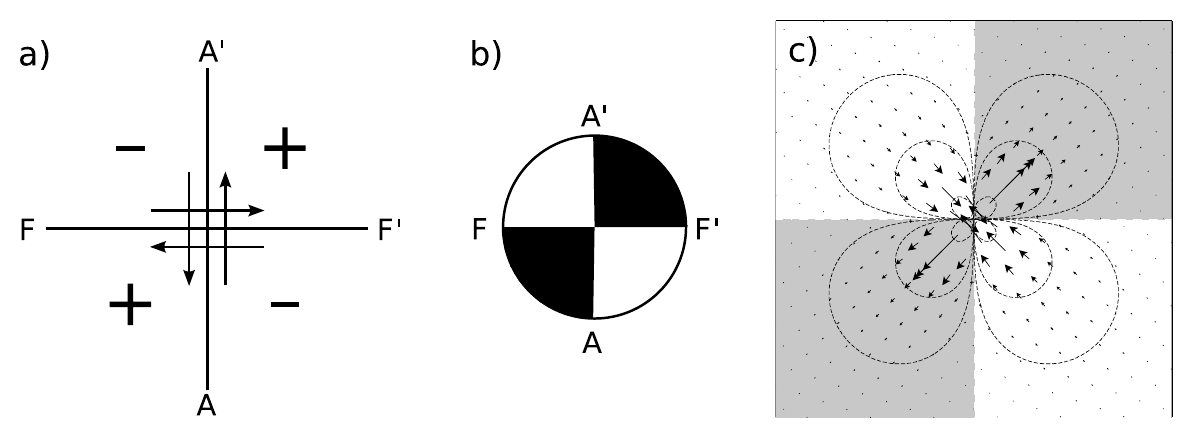
\includegraphics[width=0.90\textwidth]{figures/fig_double_couple.png}
\caption{Double couple deformation mechanism. a) Plan view of horizontal displacement
on an idealized point vertical fault A-A' or F-F' and resulting distribution
of compressions (+) and dilatations (-). b) Focal mechanism representation
on a stereographic projection. Compression quadrants are filled. c)
Horizontal displacement produced by a point size vertical dislocation
computed with the \citet{okad92} equations; compressional quadrants
are filled while dilatational are kept empty following the focal mechanism
representation. a) and b) modified from \citet{bullen}.}

\label{fig1}
\end{figure}

The most used representation of the double couple is based on the
stereographic projection. In this projection both nodal planes of
the focal mechanism are plotted, and the quadrants containing the
T axis, the compression quadrants, are filled (Figure \ref{fig1}).
This kind of representation - commonly called ``beach-ball'' - located
on a map on the earthquake epicenter is useful to interpret the seismic
data from a tectonic point of view, allowing the study of the earthquake
and its rupture fault plane on its tectonic context, being one of
the basis of the seismotectonics. The compressional and dilatational
quadrants are separated by two orthogonal planes, the nodal planes,
being one of them the plane of rupture that generated the earthquake
(Figure \ref{fig2}).

As we increase the number of focal mechanisms to study, we increase
the difficulty to interpret the data, obscuring frequently the details
of a tectonic environment if we just project them over a map. In order
to facilitate the study of groups of focal mechanisms several plots
can be proposed, great part of them based on classical structural
geology plots.

\begin{figure}
\centering
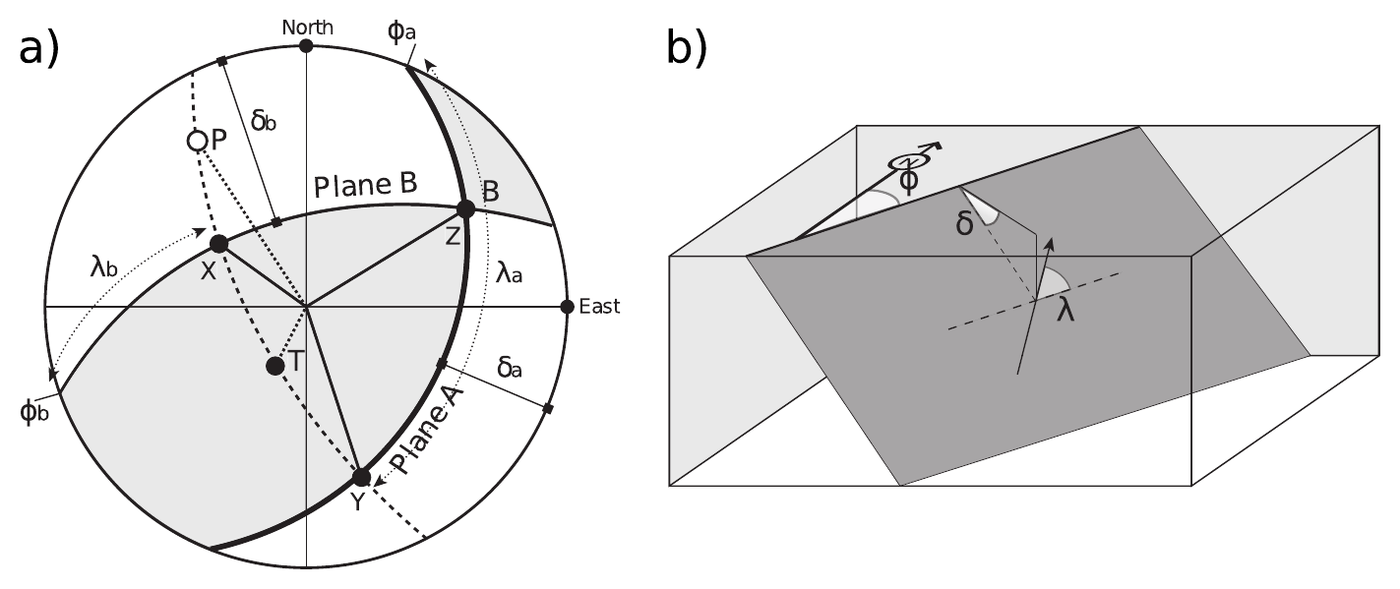
\includegraphics[width=0.95\textwidth]{figures/fig_focal_sphere.png}
\caption{a) Focal sphere diagram on stereographic projection on the lower hemisphere.
Nodal planes A and B, A representing the fault plane and B the auxiliary
plane, with its orientation characteristics: $\varphi$, strike; $\delta$,
dip and $\lambda$, rake. The orientation of the SMT principal axes
are also shown: T, B and P. Modified from \citet{udia89}. b) Block
diagram showing the parameters that define the orientation of a fault
plane in the space: $\varphi$, strike; $\delta$, dip and $\lambda$,
rake.}
\label{fig2}

\end{figure}

The plots inherited from the structural geology are based in the geometrical
characteristics of the nodal planes of the SMT, equivalent to the
characteristics of the fault planes: strike ($\varphi$), dip ($\delta$)
and rake ($\lambda$) (Figure \ref{fig2}). The main problem of these
representations is the duplication of data. Each focal mechanism presents
two equivalent and orthogonal nodal planes. The selection of one of
them as the fault plane is not straightforward and although from a
mechanical point of view they can be discriminated \citep{mcke69,mich87,geph90},
when both nodal planes are mechanically compatible or reactivated
structures can be present, additional geological and/or geophysical
information is required. There are as many representations of this
kind as possible combinations between these parameters and its derivatives
(usually trigonometrical functions). These relations can be represented
in biaxial plots or stereographic projections \citep[e.g.][]{davi96,rams97,poll05}.

The focal mechanisms can also be plotted as function of the principal
axes T, B and P. These axes form an orthogonal system. The orientation
of each axis can be defined in the space as any line, by its direction
and plunge. The main advantages of these representations are: the
univocality, each focal mechanism is represented by one point; its
simplicity of interpretation, the kind of deformation (normal, reverse,
strike-slip) is function of the plunge of the axes; and the reduction
of errors compared with the planes, as they are derived from the principal
axes of the SMT \citep{vann03}.

\section{Parameters computed by FMC}
\label{sec:parameters-computed-by-fmc}

This section describes how FMC obtains each of the parameters listed in
section~\ref{sec:output}.

\textbf{Moment tensor.} FMC works internally in the \citet{aki80} Cartesian system (\(x\) north,
\(y\) east, \(z\) down). The Harvard components (\(r\) up, \(\theta\) south, \(\phi\) east) are
converted as:

\[
\mathbf{M} = \begin{pmatrix} M_{\theta\theta} & -M_{\theta\phi} & M_{r\theta} \\ -M_{\theta\phi} & M_{\phi\phi} & -M_{r\phi} \\ M_{r\theta} & -M_{r\phi} & M_{rr} \end{pmatrix}
\]

With \texttt{AR}, \texttt{P} and \texttt{PT} input, a double-couple tensor is built from the unit
normal \(\mathbf{n}\) and slip \(\mathbf{d}\) vectors of nodal plane A as
\(M_{ij} = M_0\,(d_i n_j + d_j n_i)\).

\textbf{Principal axes.} The eigenvalues \(\lambda_1 \le \lambda_2 \le \lambda_3\) of \(\mathbf{M}\)
and their eigenvectors define the P, B and T axes respectively. The trend (azimuth, 0--360°) and
plunge (0--90°, downwards) of each axis are given.

\textbf{Nodal planes and slip vectors.} The unit normal and slip vectors of the nodal planes are
obtained from the P and T unit vectors as \(\mathbf{n} \propto \mathbf{T}+\mathbf{P}\) and
\(\mathbf{d} \propto \mathbf{T}-\mathbf{P}\); exchanging both vectors gives the other nodal plane.
Strike, dip and rake follow the \citet{aki80} convention. The trend of the slip vector of each plane
is its azimuth, and its plunge is

\[
\text{plunge} = \arcsin(\sin\lambda\,\sin\delta),
\]

positive for slip with a reverse component (rake \textgreater{} 0) and negative for slip with a
normal component (rake \textless{} 0).

\textbf{Scalar seismic moment and magnitude.} The scalar moment is computed following
\citet{silv82}, and the moment magnitude following \citet{hank79}, with \(M_0\) in dyn·cm:

\[
M_0 = \sqrt{\frac{\lambda_1^2+\lambda_2^2+\lambda_3^2}{2}}, \qquad M_w = \frac{2}{3}\log_{10} M_0 - 10.7333
\]

With \texttt{AR} input, \(M_0\) is obtained from Mw by inverting this relation; with \texttt{P}
input it is read from the mantissa and exponent.

\textbf{CLVD ratio and \(\Gamma\) index.} Both are computed from the eigenvalues of the deviatoric
part of the moment tensor, \(\lambda_P \le \lambda_B \le \lambda_T\), so they are not affected by
the isotropic component:

\[
f_{\mathrm{clvd}} = -\frac{\lambda_B}{\max\left(\lvert\lambda_T\rvert, \lvert\lambda_P\rvert\right)}, \qquad
\Gamma = \frac{3\sqrt{6}\,\lambda_T\lambda_B\lambda_P}{\left(\lambda_T^2+\lambda_B^2+\lambda_P^2\right)^{3/2}} .
\]

\texttt{fclvd} \citep{froh99} ranges from −0.5 to 0.5 and \texttt{Gamma} \citep{kaga85} from −1 to
1. Both are 0 for a double couple, positive for a tension-dominated CLVD,
\((\lambda_T,\lambda_B,\lambda_P)\propto(2,-1,-1)\), and negative for a compression-dominated one,
\(\propto(1,1,-2)\). This is also the CLVD sign of the source-type diagram \citep{huds89,vavr15},
where positive values plot on the left:

\begin{longtable}{p{0.223\linewidth}p{0.091\linewidth}p{0.091\linewidth}p{0.116\linewidth}p{0.306\linewidth}}
\toprule
\textbf{Source} & \textbf{\texttt{fclvd}} & \textbf{\texttt{Gamma}} & \textbf{\texttt{u\_Hudson}} & \textbf{Position in the source-type diagram} \\
\midrule
\endhead
Positive CLVD (tension-dominated) & +0.5 & +1 & −1 & left corner, ``CLVD (+)'' \\
Double couple & 0 & 0 & 0 & centre \\
Negative CLVD (compression-dominated) & −0.5 & −1 & +1 & right corner, ``CLVD (−)'' \\
\bottomrule
\end{longtable}

Other definitions differ in sign or scale, so check the convention before comparing values:
\citet{giar84} uses the opposite sign of \texttt{fclvd} (also the \(\epsilon\) of \citealp{tape12});
the \(C_{\mathrm{CLVD}}\) of \citet{vavr15} equals \(2 f_{\mathrm{clvd}}\) for deviatoric tensors;
and \(\Gamma\) is not linear in \texttt{fclvd} (\(\Gamma \approx 2.6 f_{\mathrm{clvd}}\) for small
values). \citet{kaga85} caution that the accuracy of catalogue solutions is too low to interpret
small CLVD values in terms of source complexity. Since they describe only the deviatoric part, for
tensors with a dominant isotropic component they should be read together with \texttt{fiso} and the
source-type diagram.

\textbf{Isotropic component.} The isotropic component is one third of the trace of the tensor,
\(\mathrm{iso} = \mathrm{tr}(\mathbf{M})/3\) (dyn·cm), and its ratio to the scalar moment is
\(f_{\mathrm{iso}} = \mathrm{iso}/M_0\). Global CMT solutions are constrained to be deviatoric, so
for them these values are zero within the rounding of the input data.

\textbf{Position on the diagrams.} The coordinates on the classification diagram (\texttt{x\_kav},
\texttt{y\_kav}) are described in section~\ref{sec:diagram}, and those on the
source-type diagram (\texttt{u\_Hudson}, \texttt{v\_Hudson}) in
section~\ref{sec:the-source-type-diagram}.

\textbf{Note on results from older versions.} Since version 1.10, \texttt{fclvd} has the opposite
sign to versions 1.8.1 to 1.9.1 (definition of \citealp{giar84}), so old values must be multiplied
by −1; it is also computed from the deviatoric eigenvalues, which changes it slightly (up to 0.005
in the Global CMT test data) when the input tensor has a non-zero trace. Before version 1.8.1 it was
an absolute value \citep{froh92}, and earlier versions computed the scalar moment as the average of
the absolute largest and smallest eigenvalues \citep{dzie81}, so small differences in \texttt{Mo},
\texttt{mant} and \texttt{Mw} are also expected when comparing with those versions.

\section{Diagram}
\label{sec:diagram}

\citet{froh92} developed a ternary diagram to represent focal mechanisms
based in the trigonometrical relation: 
\begin{equation}
\sin^{2}\iota_{T}+\sin^{2}\iota_{B}+\sin^{2}\iota_{P}=1,
\end{equation}
where $\iota_{T}$, $\iota_{B}$ and $\iota_{P}$ are the plunges
of the axis T, B and P of the SMT. This relation is true for three
orthogonal axes.

As the equation of a sphere with radius unity is 
\begin{equation}
x^{2}+y^{2}+z^{2}=1
\end{equation}
and all the plunge angles are positive between 0°and 90°, then the
representation of a focal mechanism defined by these axes is equivalent
to the projection of a point in an spherical octant over a planar
surface. As a sphere is not a developable surface can not be projected
onto a plane without distortion.

The projection used by \citet{froh92} represents this spherical octant
as a triangle, which is equivalent to the gnomonic geographical projection.
In this projection we define the angles 
\begin{equation}
\psi=\arctan\left(\dfrac{\sin\iota_{T}}{\sin\iota_{P}}\right)-45^{\circ},
\end{equation}
and 
\begin{equation}
\iota_{s}=\arcsin\dfrac{1}{\sqrt{3}}=\arctan\dfrac{1}{\sqrt{2}}\approx35.26^{\circ},
\end{equation}
which is the angle of the ternary symmetry axis with the orthogonal
axes of the octant.

From these angles the $x$ and $y$ coordinates over the plane are
given by: 
\begin{align}
x&=\dfrac{\cos\iota_{B}\cdot\sin\psi}{\sin\iota_{s}\cdot\sin\iota_{B}+\cos\iota_{s}\cdot\cos\iota_{B}\cdot\cos\psi}\\
y&=\dfrac{\cos\iota_{s}\cdot\sin\iota_{B}-\sin\iota_{s}\cdot\cos\iota_{B}\cdot\cos\psi}{\sin\iota_{s}\cdot\sin\iota_{B}+\cos\iota_{s}\cdot\cos\iota_{B}\cdot\cos\psi}
\end{align}
The angle $\iota_{s}$ in the projection is the angle of the plunges
of the axes T, B and P for the focal mechanism that occupies the barycentre
of the ternary diagram where $x=y=0$.

\begin{figure}
\centering
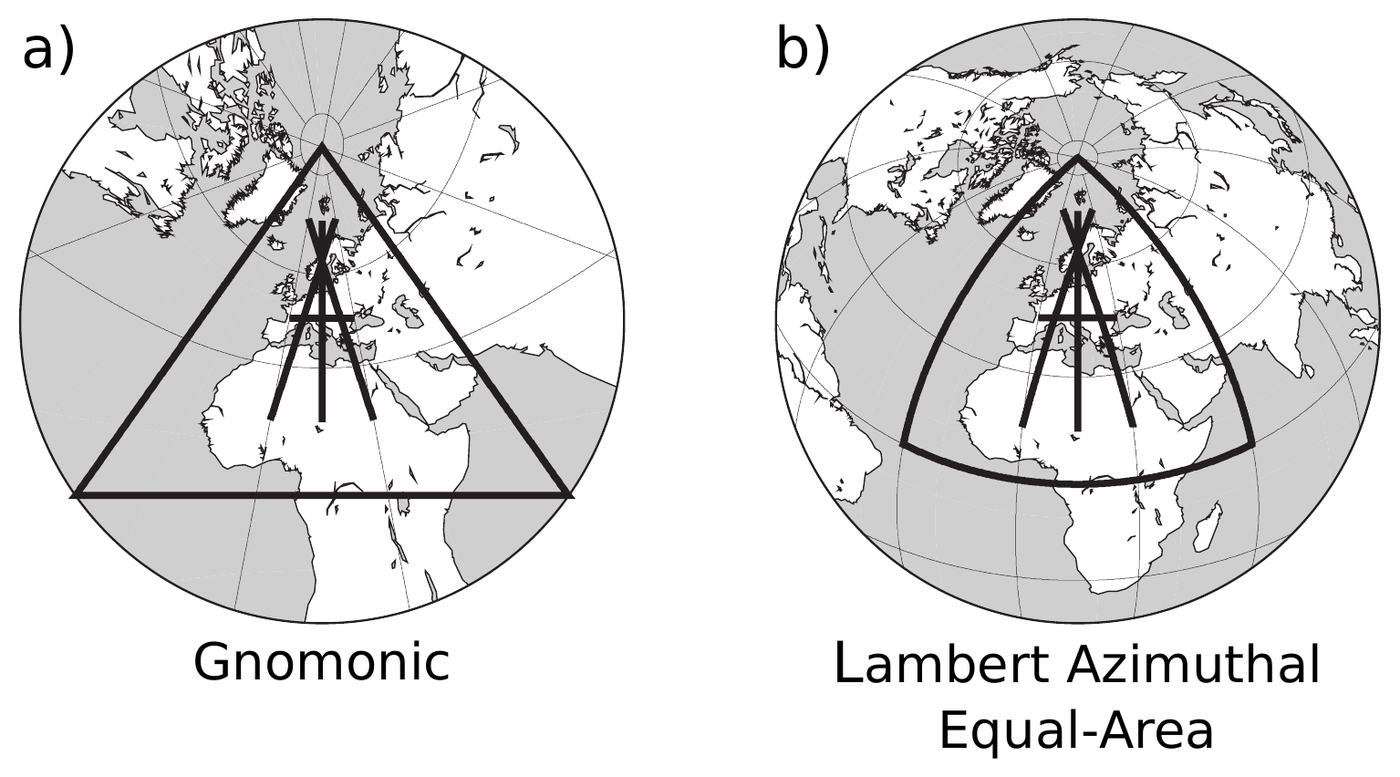
\includegraphics[width=0.88\textwidth]{figures/fig_projections.png}
\caption{Representation of an hemisphere of the globe centred on Europe (45\textdegree
N, 15\textdegree E) in the two different projections referenced in
the text: a) Gnomonic projection; b) Lambert azimuthal equal-area.
In thick lines are marked the spheric octant and some reference lines
in order to compare both projections.}
\label{fig3}
\end{figure}

As can be seen in Figure \ref{fig3}a this projection introduces remarkable
distortions towards the extremes of the diagram. This distortions
could difficult the study of some groups of focal mechanisms as the
author pointed out \citep{froh01}. In order to avoid these distortions
\citet{kave96} proposed the use of a projection capable of maintain
the proportion of the areas equal, equivalent to the Lambert azimuthal
equal-area projection (Figure \ref{fig3}b), which is the used in
structural geology to generate the stereographic equal-area Schmidt
stereonet. In this case the limits of the diagram are formed by great
circles instead of straight lines forming a triangle (Figure \ref{fig3}).

If we take the sines of the plunges of the main axes $\iota_{T}$,
$\iota_{B}$ and $\iota_{P}$:

\begin{equation}
z_{T}=\sin\iota_{T},\quad z_{P}=\sin\iota_{P},\quad z_{B}=\sin\iota_{B}
\end{equation}

the length of the vector that connects the center of the diagram with
the projected point is defined by

\begin{equation}
L=2\sin\left[\frac{1}{2}\cdot\arccos\left(\dfrac{z_{T}+z_{P}+z_{B}}{\sqrt{3}}\right)\right]
\end{equation}

and the normalization factor is:

\begin{equation}
N=\sqrt{2\cdot[(z_{B}-z_{P})^{2}+(z_{B}-z_{T})^{2}+(z_{T}-z_{P})^{2}]}
\end{equation}

The coordinates of the projected focal mechanisms in the plane are
defined as follows (these equations correct a typo present
in \citet{kaga05}):

\begin{align}
x&=\sqrt{3}\cdot\frac{L}{N}\cdot(z_{T}-z_{P})\\
y&=\frac{L}{N}\cdot(2z_{B}-z_{P}-z_{T})
\end{align}

\section{Focal Mechanism Classification}

In order to classify the focal mechanisms \citet{kaga05} divided
the octant in three areas (Figure \ref{fig4}b) corresponding to the
three basic Andersonian regimes: normal, reverse and strike-slip.
The dividing lines start at the diagram center and run through the
middle of each great circle (dashed lines in Figure \ref{fig4}b).
This classification, although simple and straightforward, is too basic
sometimes for a detailed seismotectonic study.

\begin{figure}[h]
\centering
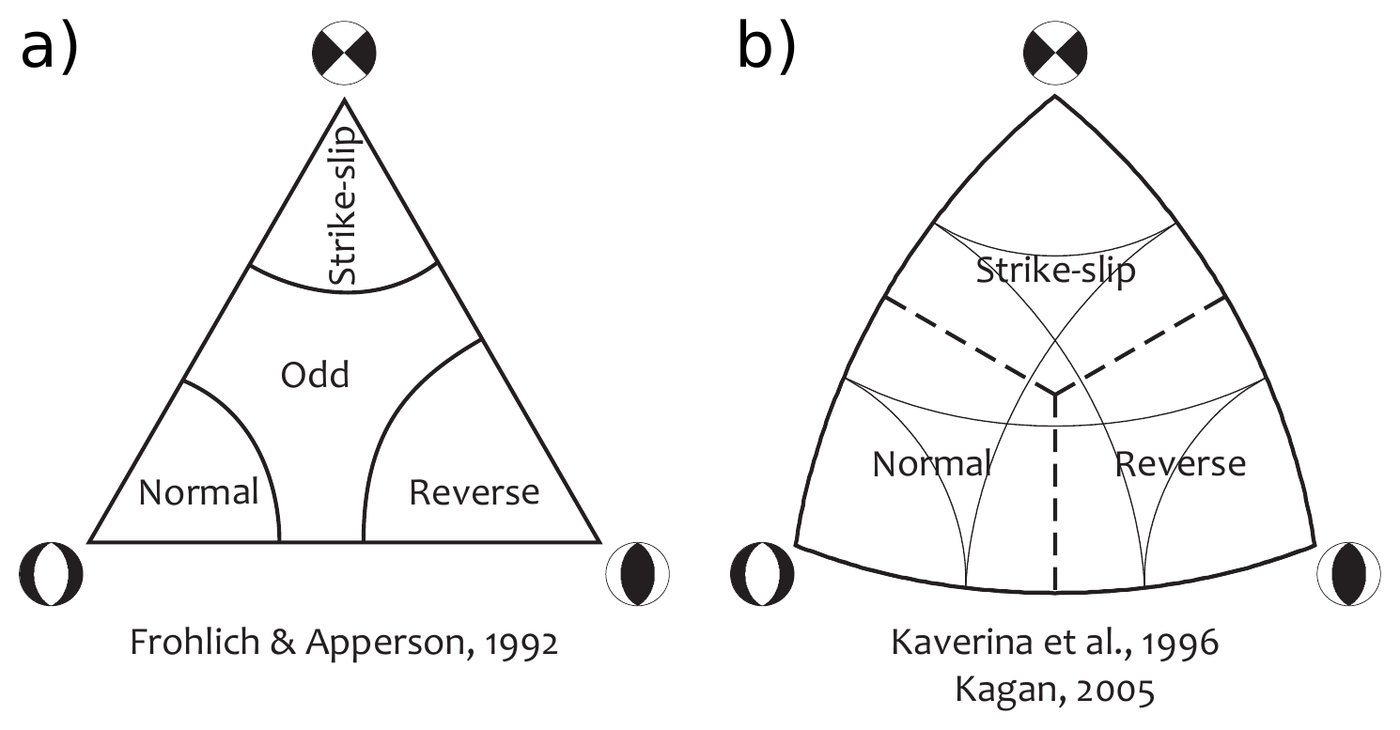
\includegraphics[width=0.88\textwidth]{figures/fig_kagan_frohlich.png}
\caption{Focal mechanisms classification diagrams based on SMT axes plunges
proposed by a) \citet{froh92} and b) \citet{kaga05}.}
\label{fig4}

\end{figure}

From the seismotectonic point of view an earthquake reflects the brittle
lithospheric strain produced by tectonic processes. The vast majority
of earthquakes are produced by displacements on faults (some other
processes as deep volume changes or cave collapses can produce seismic
signals too), and they are interpreted usually as fault ruptures.
Following this reasoning the most appropriate classification for the
focal mechanism should be done by means of the slip vector on the
fault, given by the rake angle. This classification can be done following
one of the proposed conventions \citep{rick72,aki80,ange94}. As has
been mentioned before, the problem is the duplicity of data due to
the two nodal planes solution of the focal mechanism.

An extended discussion on the relation among the different focal mechanism
parameters can be found on \citet{cele10}; the author also points
out the difficulty on interpreting the stress state from the focal
mechanisms, specially where oblique faulting takes place and reactivation
of inherited structures is possible \citep{wyss92}.

However the SMT can be interpreted as a seismic strain tensor \citep{kost74}
where the main axes are equivalent to the SMT main axes \citep{wyss92}.
With this relation in mind we can interpret the populations of focal
mechanisms as representations of strains in different tectonic settings.
Oblique slip focal mechanisms with normal component can be interpreted
as transtensional strain, while oblique slip focal mechanisms with
reverse component can be interpreted as transpressional.

In order to count with a classification more detailed than the one
of \citet{kaga05} I decided to classify the focal mechanism in a
series of fields that include the oblique slip regimes \citep{tesis}.
This approximation is similar to the \citet{EPRI} classification;
with 7 classes of earthquakes: 1) Normal; 2) Normal - Strike-slip;
3) Strike-slip - Normal; 4) Strike-slip; 5) Strike-slip - Reverse;
6) Reverse - Strike-slip and 7) Reverse. The resulting diagram incorporating
this 7 fields classification to the Kaverina projection is shown in
Figure \ref{fig5}.

\begin{figure}
\centering
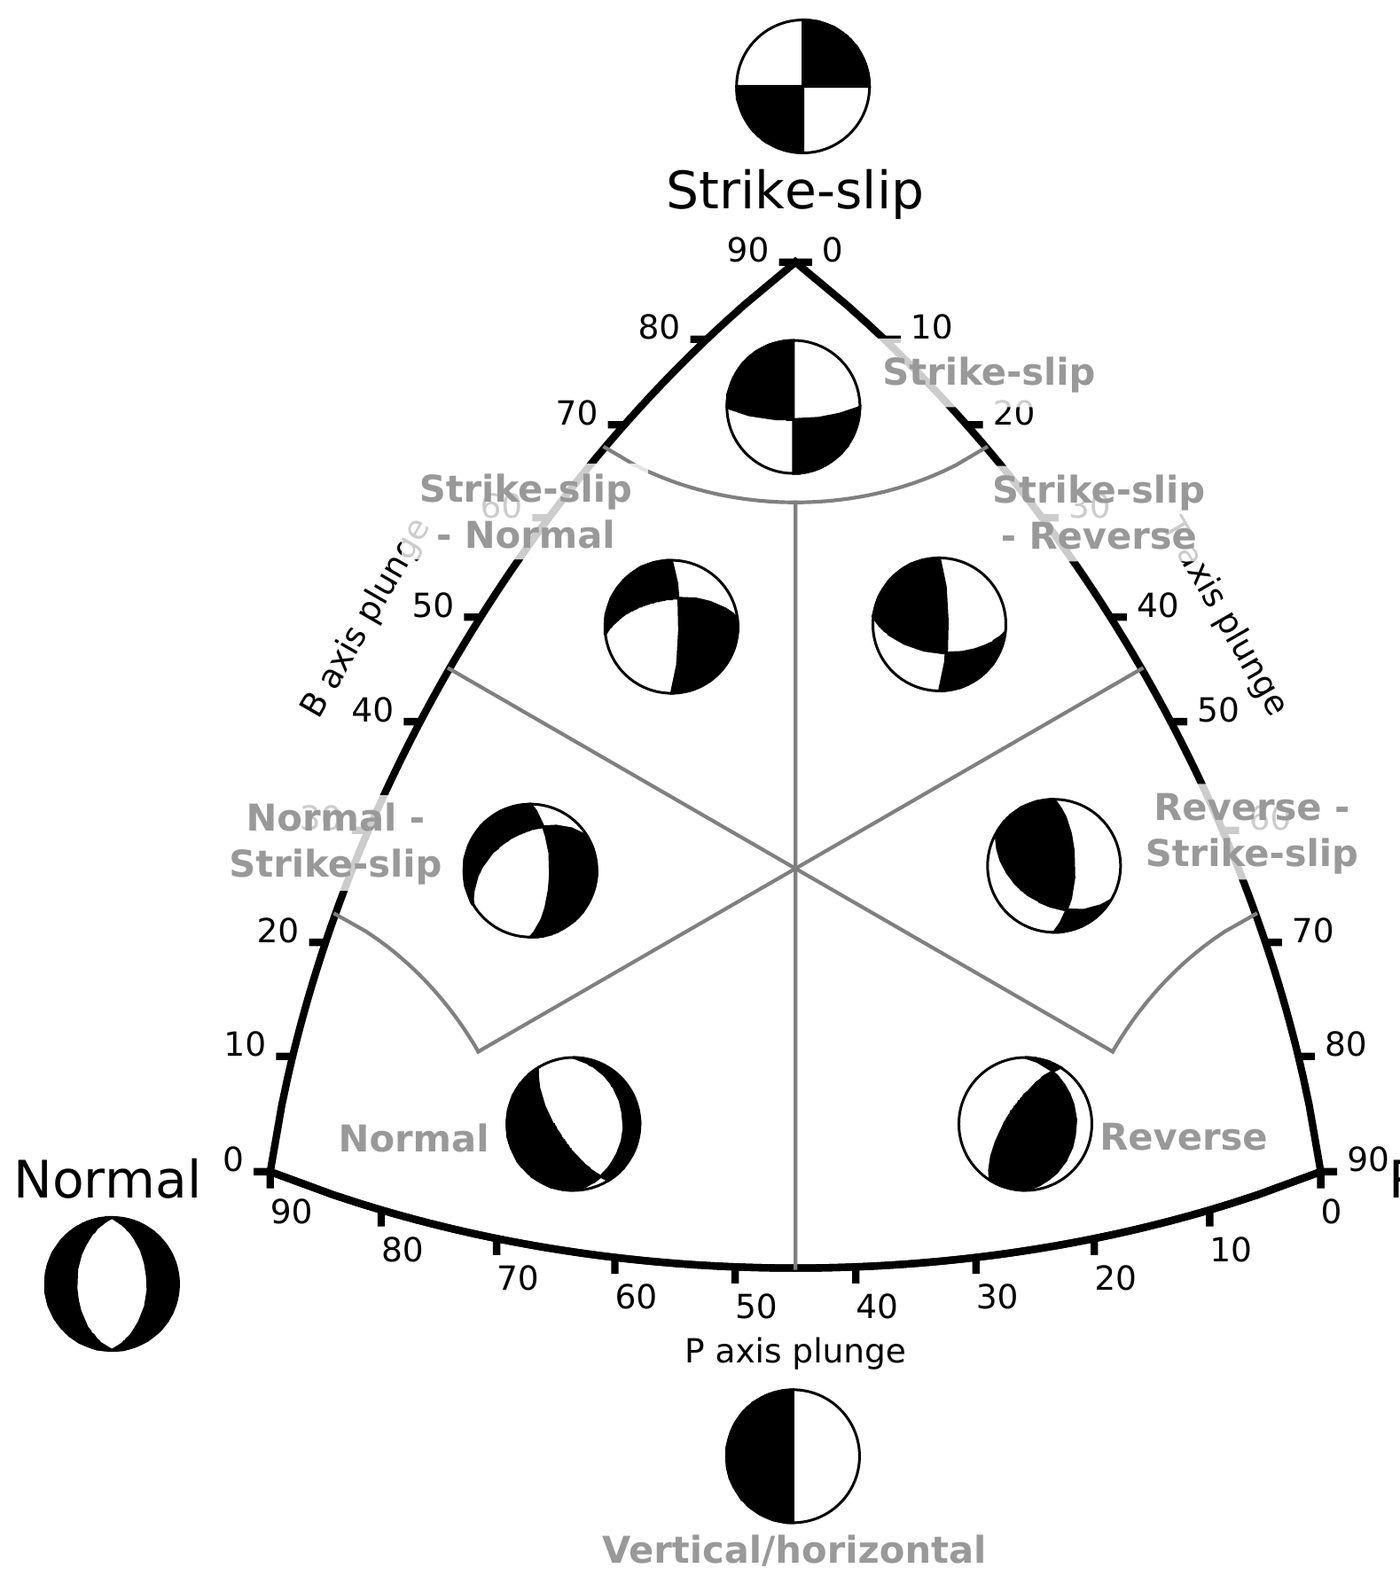
\includegraphics[width=0.72\textwidth]{figures/fig_classification_fields.png}
\caption{Focal mechanism classification diagram. N) Normal; N-SS) Normal -
Strike-slip; SS-N) Strike-slip - Normal; SS) Strike-slip; SS-R) Strike-slip
- Reverse; R-SS) Reverse - strike-slip and R) Reverse.}
\label{fig5}

\end{figure}

The algorithm to classify the focal mechanisms based on the SMT main
axes plunges is the shown in Figure \ref{fig_flow}.

When one of the three main SMT axes is greater or equal than 67.5$^{\circ}$
(resulted from $3\cdot\frac{\pi/2}{4}$) we obtain a \textquotedbl pure\textquotedbl{}
Andersonian tectonic regime. From the pure normal or reverse faulting
to the strike-slip faulting there is a range of oblique faulting types
with more or less relevance of the horizontal component. On the other
hand between the pure normal and pure reverse faulting there is a
permutation of the T and P axes in the vertical position, while the
B axis remains horizontal. The transition takes place when the P and
T axes plunge equally and a vertical nodal plane is present.

In the following section I compare the results of both classifications,
the one based in the main axes plunges of the moment tensor and the
one based on the fault rakes.

\subsection{Comparison between rake-based and SMT axes-based classifications}

In order to classify the nodal planes according to its rakes I adopted
a convention hybrid between the \citet{rick72} and \citet{aki80}
conventions. The focal mechanism rakes are usually given with the
\citet{aki80} convention, while from a geological point of view the
\citet{rick72} convention is more used. I define 7 equivalent classes
to those used in the SMT axes-based classifications (Figure \ref{fig6}).

\begin{figure}
\centering
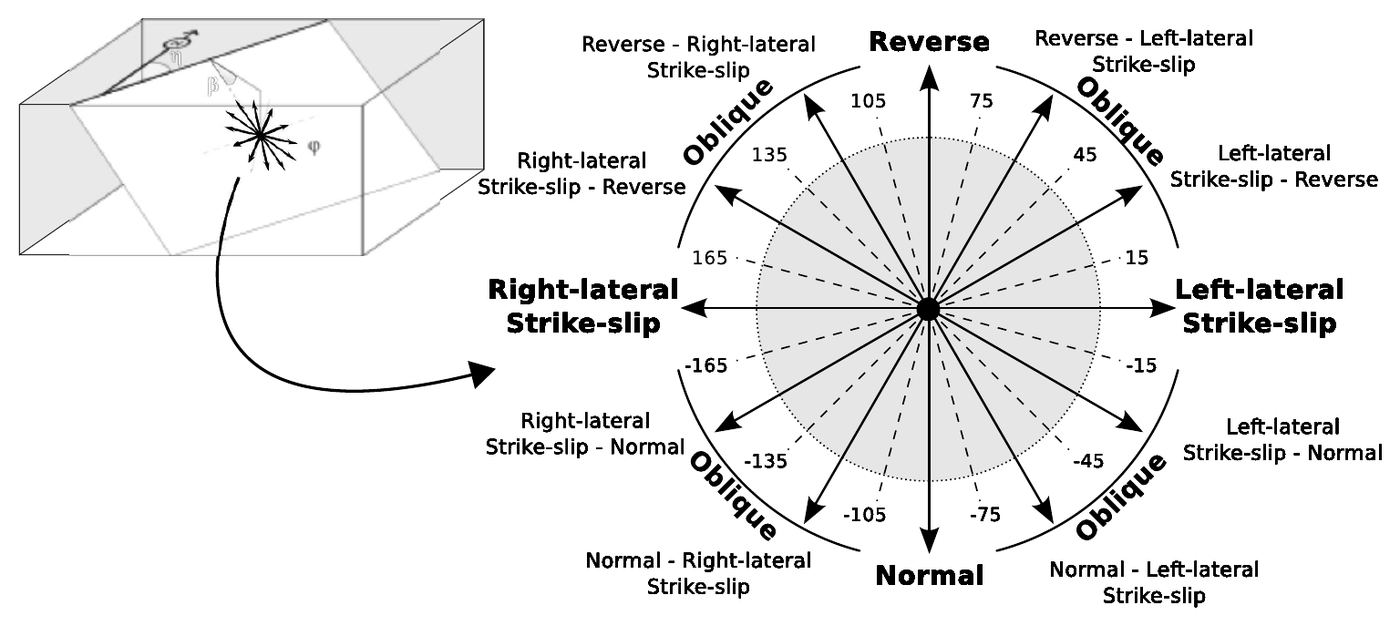
\includegraphics[width=0.95\textwidth]{figures/fig_rake_classification.png}
\caption{Diagram showing the convention used in this work for the rake classification
of faults or focal mechanism nodal planes. Inside the grey circle
the equivalent SMT axes-based classification is shown (Figure \ref{fig5}).}
\label{fig6}

\end{figure}

Each one of the nodal planes of the focal mechanisms from the Global
CMT catalog \citep{CMT} is classified according to the rake classification
shown in Figure \ref{fig6}. From the analysis of the focal mechanism
alone we cannot choose unequivocally the fault plane responsible of
the earthquake. To analyze the degree of uncertainty I show in Figure
\ref{fig7}a the relative frequency of relations between nodal planes
rupture types. For example, it can be seen that when one nodal plane
is classified as normal, the other can be normal as well, or can present
some strike-slip component, but it can not present reverse component;
the same can be said for the reverse nodal planes. When one nodal
plane is pure strike-slip, the other can present dip-slip component
too, ranging from normal with strike-slip component (N-SS) to reverse
with strike-slip component (R-SS), but being more frequent the relations
between nodal planes of mainly strike-slip type.

Comparing the focal mechanism classified with the SMT axes and the
nodal planes classified with the rakes (Figure \ref{fig7}b) a similar
picture as the described above can be seen. The percentages of relations
change sensibly, but the common picture is the same. When the focal
mechanism is classified as normal type we can expect that both nodal
planes are of normal type or normal with some strike-slip component.
Similarly when the focal mechanism is classified as reverse, both
nodal planes are mainly of the reverse type too. For the case of the
strike-slip focal mechanism almost all the nodal planes are of strike-slip
type too.

We can conclude that there is not much difference between the results
obtained from the rake classification of the nodal planes and the
classification of the focal mechanism attending to the SMT axes plunges.
The focal mechanism classification based on the SMT axes has the advantage
of the univocallity of its classification, in contrast with the duplicity
of data and uncertainty related to the nodal planes rake classification.

\begin{figure}
\centering
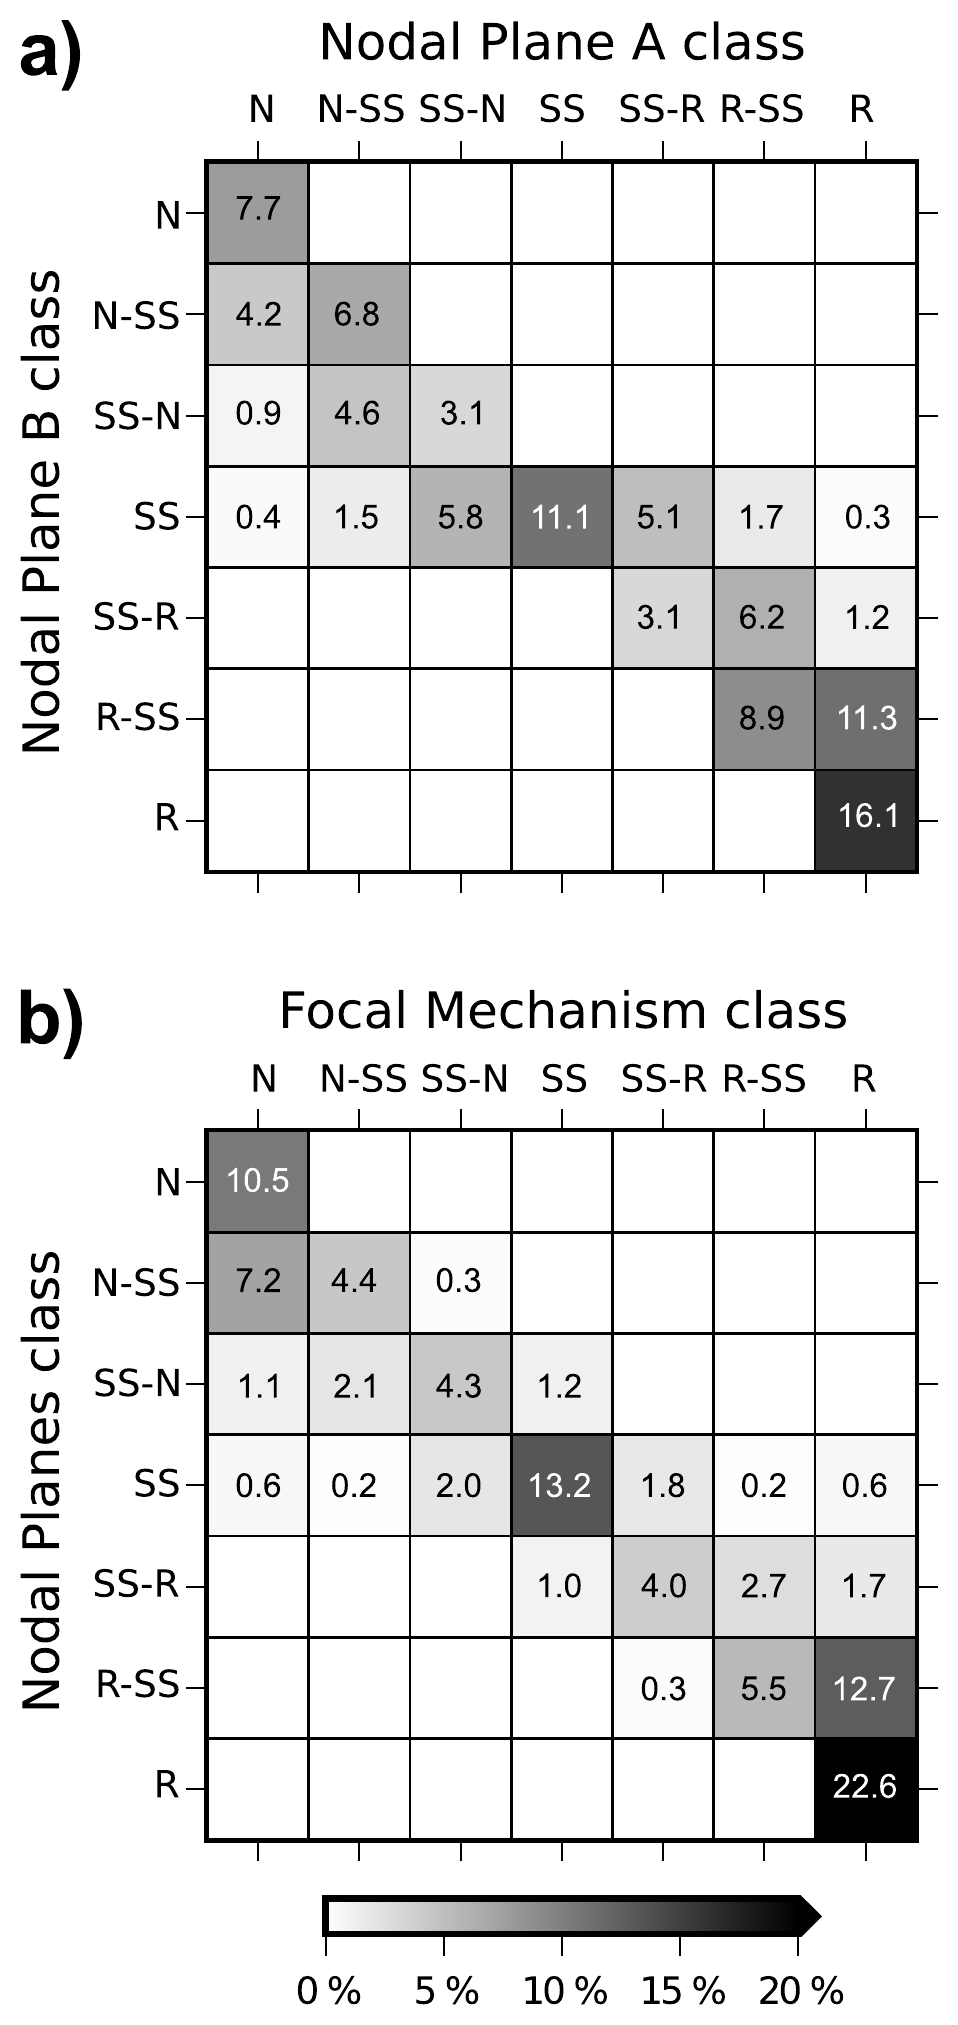
\includegraphics[width=0.48\textwidth]{figures/fig_heatmaps.png}
\caption{Heatmaps of the proportion of relations between a) both nodal planes
rupture type based on the rake classification, and b) between the
focal mechanism classification and the nodal planes rupture types
rake classification. The data used is the entire Global CMT catalog
\citep{CMT}. Numbers show percentages over the entire catalogue.}
\label{fig7}
\end{figure}

\section{The source-type diagram}
\label{sec:the-source-type-diagram}

The classification diagram describes the double-couple part of the moment tensor. To analyse the
non-double-couple components, FMC also plots the source-type diagram of \citet{huds89}, in the
skewed-diamond form described by \citet{vavr15} (flag \texttt{-pd}). The eigenvalues
\(\lambda_1 \le \lambda_2 \le \lambda_3\) are normalised by the largest absolute eigenvalue,
\(\hat\lambda_i = \lambda_i / \max_j \lvert\lambda_j\rvert\), and the coordinates are

\[
u = -\frac{2}{3}\left(\hat\lambda_1 + \hat\lambda_3 - 2\hat\lambda_2\right), \qquad v = \frac{1}{3}\left(\hat\lambda_1 + \hat\lambda_2 + \hat\lambda_3\right).
\]

The vertical coordinate \(v\) measures the isotropic component: pure explosions plot at the top
vertex (\(v=1\)) and pure implosions at the bottom one (\(v=-1\)). The horizontal coordinate \(u\)
measures the CLVD component: a pure double couple plots at the centre, and pure CLVD sources at
\(u=\pm 1\) on the horizontal axis. Because \(u\) is minus the CLVD coordinate of the standard
decomposition \citep[][eqs. 7 and 42]{vavr15}, positive CLVDs (tension-dominated) plot at the left
corner (\(u=-1\), labelled ``CLVD (+)'') and negative CLVDs (compression-dominated) at the right
corner (\(u=+1\), labelled ``CLVD (−)''). For deviatoric tensors \(v=0\) and
\(u=-2 f_{\mathrm{clvd}}\), so events with positive \texttt{fclvd} plot on the left and events with
negative \texttt{fclvd} on the right (section~\ref{sec:parameters-computed-by-fmc}). The dashed
diagonal line of the diagram joins the two lateral vertices, at \((\pm 4/3, \pm 1/3)\).

\newpage{}

\bibliographystyle{elsarticle-harv}
\phantomsection\addcontentsline{toc}{section}{\refname}\bibliography{FMC_manual}

\end{document}
